\documentclass[preprint,review,12pt]{elsarticle}

\usepackage{amsmath,amssymb}
\usepackage[T1]{fontenc}
\usepackage[utf8]{inputenc}
\usepackage{lmodern}
\usepackage{url}
\usepackage{hyperref}
\urlstyle{same}
% Bibliography entries carry bare DOIs; without this TeX has no
% legal breakpoint inside them and the paragraph cannot be set.
\PassOptionsToPackage{hyphens}{url}
\usepackage{graphicx}
\usepackage{booktabs}
\usepackage{longtable}

% pandoc emits these but does not define them.
\providecommand{\tightlist}{%
  \setlength{\itemsep}{0pt}\setlength{\parskip}{0pt}}
% pandoc's longtable preamble writes column widths as
%   p{(\columnwidth - 4\tabcolsep) * \real{0.3333}}
% which needs calc's \real, not a passthrough: defining it as the identity
% leaves "* 0.3333" as an unresolved factor and TeX loops trying to set the
% column.
\usepackage{array}
\usepackage{calc}

\journal{Structural Change and Economic Dynamics}

\begin{document}

\begin{frontmatter}

\title{From Fugitive Cash to Non-Fugitive Provisioning:\\
Redistribution Feasibility under International Settlement Constraints}

\author[anon]{[Author removed for review]\corref{cor1}}
\cortext[cor1]{Corresponding author.}
\affiliation[anon]{organization={[Removed for review]}}

\begin{abstract}
Automation is reducing labour demand across occupations and countries simultaneously --- cognitive work through large language models, physical work through autonomous machinery and robotics --- closing the traditional channel through which displaced workers move to surviving sectors and making large-scale redistribution a structural necessity. Existing models of universal basic income and cash transfers treat feasibility as a question of domestic fiscal capacity, leaving the international monetary constraint unexamined. This paper constructs a twenty-five-bloc closed-world computational model in which every import is another bloc's export and every capital outflow is another's inflow. Households allocate income across food, general consumption, and housing through a Stone--Geary demand system. Four redistributive policy regimes --- universal cash, targeted cash, food vouchers, and in-kind housing via community land trusts --- are calibrated to deliver identical welfare at introduction. A foreign-exchange settlement constraint binds non-reserve blocs: imports cannot exceed the sum of export earnings, reserves, and borrowing capacity. The model produces five findings. First, welfare-equivalent regimes generate sharply different macrofinancial footprints because their demand composition and import content differ structurally. Second, in blocs with low creditworthiness and low food self-sufficiency, universal cash transfers make recipients worse off than no transfer at all. Third, the feasible set of regimes varies by position on a creditworthiness--self-sufficiency plane, producing an institutional feasibility phase diagram. Fourth, automation amplifies this selection pressure, shrinking the feasible set and separating the regimes. Fifth, cost-of-living adjustment creates a world-price externality: each bloc's individually rational indexation collectively undermines purchasing power. The international monetary system selects not only how much redistribution a country can afford but which institutional forms can survive.
\end{abstract}


\begin{keyword}
redistribution \sep settlement constraint \sep community land trust \sep automation \sep monetary hierarchy \sep transfer modality
\end{keyword}

\end{frontmatter}

\section{Introduction}

Automation and artificial intelligence are reducing the demand for human
labour across occupations and countries simultaneously. Office work is
being restructured by large language models whose multilingual
capability allows industry-specific software built under the strict
regulatory regimes of high-income countries to diffuse rapidly into the
high-revenue segments of developing economies with minimal localisation
cost. Manufacturing is being restructured by
autonomous machinery, logistics by self-driving vehicles, and physical
services by humanoid robots and drones. Previous waves of automation
displaced one broad occupational class at a time, and the displaced
workers moved to the surviving class; this time, cognitive and physical
automation are advancing concurrently, closing the traditional
adjustment channel. These are not prospective disruptions but
extensions of changes already underway. Developing countries that have
not yet completed industrialisation face the additional pressure of
premature deindustrialisation: manufacturing employment peaks at lower
shares and lower income levels than it did for earlier developers, as
labour-saving technology and globalisation close the traditional pathway
from agriculture to industry (Rodrik, 2016). When these forces operate
concurrently across the world economy, the result is a simultaneous
contraction in labour income that no single country caused and no single
country can reverse through domestic policy alone.

When labour income falls, people must be provisioned through some other
channel. The question is not whether redistribution will be needed ---
it will --- but whether every country can sustain it. A government that
can neither restore employment nor deliver transfers loses credibility.
Economic collapse and political instability do not follow a fixed
sequence: default may precede civil disorder, or civil disorder may
destroy the economy that sustains the state. In either case, the
consequences do not remain within national borders. They take the form
of armed conflict, coercive migration, or refugee flows that impose
costs on neighbouring and distant states alike. Preventing this outcome
at multiple points across the world economy simultaneously is the
problem that motivates this research.

The dominant framework for analysing redistribution treats it as a
question of domestic fiscal capacity. Models of universal basic income
(UBI) and other cash transfers typically operate within a closed economy
or a single small open economy facing an exogenous rest of the world.
They ask whether tax revenue can cover the transfer, what happens to
labour supply, and how the income distribution shifts (Daruich and
Fernández, 2024; Luduvice, 2024; Banerjee, Niehaus, and Suri, 2019;
Coady and Prady, 2018). Even heterodox approaches that recognise the
external constraint --- the post-Keynesian literature on monetary
sovereignty and currency hierarchy --- have directed their analysis at
the job guarantee rather than at cash or in-kind transfers (Bonizzi,
Kaltenbrunner, and Michell, 2019; Prates, 2020; Vernengo and Pérez
Caldentey, 2019). The international dimension of redistribution remains
largely unexamined. Yet for any country that imports a significant share
of its food, energy, or capital goods, the fiscal cost of a transfer is
only part of the story. The transfer generates demand, part of which
falls on imports. Imports require foreign exchange. Foreign exchange
requires export earnings, reserves, or borrowing --- and borrowing
capacity depends on the country's position in the international monetary
hierarchy. A transfer that looks affordable in domestic-budget terms can
become self-defeating when its import content encounters a binding
settlement constraint.

The institutional form of the transfer compounds this problem. Cash and
in-kind provisioning are not interchangeable even when they achieve the
same welfare gain at the moment of introduction. A cash transfer enters
the recipient's budget and is spent according to the recipient's
preferences, which in an import-dependent economy means a substantial
fraction leaks into traded-goods demand and, through that channel, into
foreign-exchange requirements. An in-kind housing provision ---
represented in this paper by a community land trust (CLT) that supplies
housing as a physical asset rather than a monetary entitlement ---
removes land rent from the transfer cost, reduces the import content of
the provisioning, and preserves its real value regardless of domestic
price movements. The recipient is housed whether the currency
depreciates or not. This is not an argument that in-kind provision is
universally superior: it is confined to housing, it does not address
food, and it carries costs in quality, location, and spatial
concentration that the model does not measure. But the macrofinancial
footprint of the two modalities differs, and that difference interacts
with the settlement constraint in ways that existing models do not
capture.

No published model, to our knowledge, places these elements together.
The UBI literature lacks a closed multi-country world in which one
country's transfer spending changes another country's import prices. The
currency-dominance literature derives the reserve-currency advantage
from trade-finance complementarities (Gopinath and Stein, 2021) or
safe-asset demand (Farhi and Maggiori, 2018), but does not trace the
advantage through to social-transfer feasibility. The
automation-and-redistribution literature recognises that AI may
deteriorate the terms of trade for developing countries (Korinek and
Stiglitz, 2021) but treats the adjustment as a relative-price channel,
not a hard settlement constraint. Two recent unpublished studies --- a
New Keynesian small open-economy model of scaled cash transfers (Mendes,
Miyamoto, Nguyen, and Pennings, 2026) and an agent-based
stock-flow-consistent model of post-automation UBI (Wossnig, 2026) ---
occupy adjacent territory but differ in structure: neither closes the
world, neither maps modality viability as a function of structural
position, and neither derives monetary-hierarchy asymmetry from
settlement mechanics.

This paper constructs a multi-bloc dynamic computational model that
fills this gap. Twenty-five economic blocs, positioned on a
two-dimensional plane defined by creditworthiness and food
self-sufficiency, trade in a closed world where every import is another
bloc's export and every capital outflow is another's inflow. Households
allocate income and transfers across food, general consumption, and
housing through a Stone--Geary demand system. Four redistributive policy
regimes --- universal cash, targeted cash, food vouchers, and in-kind
housing --- are calibrated to deliver the same welfare at introduction.
A foreign-exchange settlement constraint binds non-reserve blocs: they
can import only what they can pay for with export earnings, reserves,
and borrowing. A post-employment transition, driven by a single
automation parameter, simultaneously raises productive capacity, lowers
unit costs, reduces labour income, and shifts income toward capital ---
forcing the question of whether transfers can fill the gap before the
settlement constraint closes it.

The model produces five principal findings. First, welfare-equivalent
policy regimes generate sharply different macrofinancial footprints:
in-kind housing requires less fiscal outlay and less import demand than
cash for the same welfare gain, not because leakage was assigned a lower
coefficient but because the demand composition and price-transmission
channels differ structurally. Second, in blocs with low creditworthiness
and low self-sufficiency, universal cash transfers make recipients worse
off than no transfer at all: the exchange-rate depreciation and
import-price increase caused by the transfer exceed the transfer's
value. Third, the feasibility of each modality depends on the bloc's
position on the creditworthiness--self-sufficiency plane, producing a
phase diagram in which the set of viable redistributive institutions
varies by structural position. Fourth, post-employment transition
amplifies this selection pressure: as automation rises, the feasible set
shrinks and the modalities separate. Fifth, cost-of-living adjustment of
transfers creates a world-price externality: each bloc's decision to
index its transfers to domestic prices raises traded-goods demand, which
raises import prices for all blocs --- including the adjusting bloc
itself --- so that the individually rational choice to protect
recipients' purchasing power collectively undermines it.

The paper contributes to the literature in five specific ways. It
provides, to our knowledge, the first closed-world model of
redistribution under foreign-exchange settlement constraints, filling a
gap between the domestic-fiscal UBI literature and the open-economy
currency-hierarchy literature. It maps the viability of transfer
modalities as a function of structural position --- creditworthiness and
self-sufficiency --- rather than treating feasibility as a single
national threshold. It derives monetary-hierarchy asymmetry from
settlement mechanics rather than from parametric privilege, showing that
the reserve-currency bloc's protection is conditional and disappears as
the transfer level rises. It demonstrates a world-price externality of
cost-of-living-adjusted transfers that has not, to our knowledge,
previously been shown in simulation. And it connects the post-employment
transition to the institutional selection pressure that the
international monetary system imposes on redistribution.

The remainder of the paper is organised as follows. Section 2 reviews
the relevant literature across three domains: open-economy constraints
on redistribution, transfer modality and provisioning, and
post-employment redistribution. Section 3 presents the model as a
complete system. Section 4 reports the results in five stages. Section 5
examines robustness. Section 6 discusses the implications, including the
direction of an exit through locally optimised intensive agriculture.
Section 7 states limitations. Section 8 concludes.

\section{Literature and Conceptual Framework}

\subsection{Redistribution under open-economy constraints}

The macroeconomic constraints on redistribution in an open economy have
been studied extensively, but almost never in connection with the design
of social transfers. The Mundell--Fleming framework established that a
small open economy cannot simultaneously maintain a fixed exchange rate,
free capital mobility, and an independent monetary policy --- the
so-called impossible trinity. This result has become the textbook
framing for international macroeconomic policy, yet the redistribution
literature has largely proceeded as though the constraint does not
exist. The standard UBI model operates within a single economy, asks
whether tax revenue can cover the transfer, and evaluates the effects on
labour supply and the income distribution, without modelling the
exchange rate, the current account, or the foreign-exchange position
that determines whether the country can actually pay for the imports its
transfer recipients will demand.

The balance-of-payments constraint on growth, formalised by Thirlwall
(1979) and extended to include capital flows by Thirlwall and Hussain
(1982), provides a more relevant starting point. In this framework, a
country's long-run growth rate is bounded by the ratio of its export
growth to the income elasticity of its imports. Any fiscal expansion
that raises demand --- including a large-scale cash transfer ---
increases imports and tightens the external constraint unless exports
grow commensurately. The two-gap models of Chenery and Strout (1966),
which distinguished a savings gap from a foreign-exchange gap, are the
classical ancestor of the settlement constraint used in this paper: when
the binding constraint is foreign exchange rather than domestic savings,
the country cannot spend its way to higher output regardless of its
fiscal capacity.

The structural inability of many countries to borrow in their own
currency --- Eichengreen and Hausmann's (1999) ``original sin'' ---
compounds this problem. Eichengreen, Hausmann, and Panizza (2005) showed
that original sin correlates with country size rather than with
institutional quality or fiscal discipline, which implies that the
constraint is structural and not easily removed by policy reform.
Countries that cannot borrow externally in their own currency face a
currency mismatch: depreciation raises the domestic-currency cost of
servicing foreign debt, creating a feedback loop between the exchange
rate and the fiscal position. Hausmann and Panizza (2003) found that
original sin is robustly associated only with economic size, supporting
the treatment of creditworthiness as a structural attribute rather than
a policy variable.

The post-Keynesian literature on currency hierarchy places these
constraints within a broader framework. De Paula, Fritz, and Prates
(2017) argued that the international monetary system is hierarchically
ordered, with non-reserve currencies facing structural disadvantages in
capital flows, interest-rate setting, and exchange-rate management.
Bonizzi, Kaltenbrunner, and Michell (2019) applied this framework to
critique modern monetary theory (MMT), arguing that external constraints
bind over any plausible policy horizon for developing countries. Prates
(2020) proposed that monetary sovereignty itself is a spectrum,
determined by the currency's position in the international hierarchy.
These arguments are conceptual allies of the present paper, but they
target the job guarantee and MMT, not cash or in-kind transfers, and
they do not model the transmission from transfer design to external
balance.

A separate literature has made the dominance of the US dollar
endogenous. Gopinath and Stein (2021) showed that the invoicing role and
the safe-asset role of the dollar are complementary, producing a
self-reinforcing equilibrium in which a single currency dominates even
when multiple large economies share similar fundamentals. Chahrour and
Valchev (2022) derived dollar durability from the need to finance
international trade, demonstrating multiple stable steady states. Farhi
and Maggiori (2018) located the privilege in the monopoly issuance of
safe assets. These models explain why currency dominance persists, but
none of them traces the consequence through to the feasibility of
different forms of social provisioning. The present paper derives
asymmetry from a different mechanism --- hard settlement feasibility,
defined as the accounting constraint that a country cannot import more
than it can pay for --- and connects it to the modality of
redistribution.

\subsection{Transfer modality, provisioning, and decommodification}

The macroeconomic literature on cash transfers has produced a robust
body of evidence on local price effects, labour supply, and poverty
reduction, but it has not addressed the import content or
foreign-exchange consequences of different transfer designs. Egger,
Haushofer, Miguel, Niehaus, and Walker (2022) found that a cash transfer
amounting to more than fifteen percent of local GDP in rural Kenya
produced minimal price inflation and a local multiplier of approximately
2.5. This result is widely cited as evidence that large cash transfers
are not inflationary. However, the transfers were financed by an
external NGO --- effectively a foreign-exchange inflow --- so the
settlement constraint was pre-financed. The result supports the present
paper's argument rather than contradicting it: the benign outcome
depends on a condition that domestically financed national-scale
transfers do not meet.

The comparison between cash and in-kind transfers has been studied
primarily through the lens of consumption efficiency and targeting.
Cunha, De Giorgi, and Jayachandran (2019) found that in Mexican
villages, cash transfers produced no detectable price increase while
in-kind food transfers lowered prices of the transferred goods by 3.7
percent. The authors noted that price effects were largest where local
markets were less integrated with outside markets, demonstrating that
transfer modality interacts with market openness. Currie and Gahvari
(2008) surveyed the theoretical literature on cash versus in-kind
transfers, identifying paternalism, targeting, and political economy as
the standard justifications for in-kind provision. The import content of
different modalities --- the share of spending that generates
foreign-exchange demand --- has not been systematically studied.

The incidence of demand-side housing subsidies is contested and depends
heavily on housing supply elasticity. Susin (2002) estimated that
housing vouchers raised rents by sixteen percent on average in the
ninety largest US metropolitan areas, producing a net welfare loss for
non-recipient low-income households. Fack (2006) found that in France,
seventy-eight cents of each additional euro of housing benefit was
captured by landlords through higher rents for new claimants. By
contrast, Eriksen and Ross (2015) found no effect on overall US rents,
though prices rose for units near the voucher ceiling in cities with
inelastic supply. Eerola and Lyytikäinen (2021) found no significant
pass-through in Finland. The evidence implies that rent capture is
conditional on supply elasticity --- precisely the land-constrained
urban setting in which the provisioning problem is most acute.

Community land trusts represent one institutional response to this
problem. By retaining ownership of the land and leasing it to residents,
a CLT removes ``the most rapidly appreciating element of housing'' from
the household's cost (Bourassa, 2007). Thaden and Rosenberg (2010)
documented that CLT foreclosure and delinquency rates remained low
through the 2008--2010 US housing crisis, providing evidence that the
model preserves value through macroeconomic shocks. However, the CLT
literature is almost entirely institutional and domestic. No study
examines the macroeconomic, fiscal, or open-economy properties of CLTs.
The present paper treats the CLT not as a specific institutional
prescription but as a representative case of non-cash, asset-based
provisioning --- a class of transfers whose real value does not depend
on the exchange rate and whose import content differs structurally from
that of cash.

The claim that in-kind provision is cheaper than cash is not
straightforward. Olsen (2003) showed that US public housing production
programmes cost substantially more per unit of housing service than
vouchers. The advantage claimed in this paper is therefore not
construction cost but two other properties: the exclusion of land rent
from the ongoing transfer cost, and the insulation from settlement
constraints that follows from reduced import content. These are
macrofinancial properties, not microeconomic efficiency claims.

The classical transfer problem, debated by Keynes (1929) and Ohlin
(1929), asked whether an international income transfer worsens the
paying country's terms of trade --- a ``secondary burden'' beyond the
transfer itself. Chichilnisky (1980) extended the framework to a
North--South model with basic goods, contrasting commodity transfers
with income transfers. The present paper reframes the transfer problem
for domestic social transfers whose spending leaks abroad through
imports. In an import-dependent country, a cash transfer to domestic
residents functions as an implicit international transfer to the
countries that supply traded goods. The terms ``fugitive'' and
``non-fugitive,'' introduced here, distinguish transfer modalities by
this property: a fugitive transfer is one whose value can be dissipated
through exchange-rate depreciation and import-price increases before it
reaches the recipient in real terms; a non-fugitive transfer is one
whose real value is embodied in a physical asset that is not exposed to
these channels. No prior literature uses this terminology.

\subsection{Post-employment redistribution and the missing international dimension}

The literature on automation, labour displacement, and redistribution
has grown rapidly but remains predominantly domestic in scope. Acemoglu
and Restrepo (2018) modelled the race between displacement and new task
creation in a single economy. Autor (2015) documented the historical
capacity of labour markets to generate new occupations, though recent
work acknowledges that AI may displace cognitive tasks at a pace that
exceeds historical precedent. Sachs and Kotlikoff (2012) showed that in
a closed overlapping-generations model, smart machines can produce
``immiserating growth'' in which output rises while wages and welfare
fall. None of these models addresses the international transmission of
displacement or the foreign-exchange consequences of the redistribution
it necessitates.

Korinek and Stiglitz (2021) provided the most direct treatment of the
international dimension. They argued that AI and automation may
deteriorate the terms of trade for developing countries by devaluing the
sources of their comparative advantage --- labour and natural resources.
Their analysis implies that domestic policy measures may be insufficient
to provide compensation when the terms-of-trade shift is large enough.
However, the mechanism operates through relative prices, not through
hard settlement constraints, and the analysis does not model the choice
between transfer modalities. Alonso, Berg, Kothari, Papageorgiou, and
Rehman (2022) constructed a two-country model in which robot
productivity gains favour high-wage countries and capital flows
``uphill,'' but included no redistribution or settlement mechanism.

The gap this paper addresses lies at the intersection of three
literatures that have not been connected. The post-employment literature
recognises that labour-income replacement is a structural necessity. The
currency-hierarchy literature recognises that external constraints bind
for most countries. The transfer-modality literature recognises that the
form of a transfer affects its economic consequences. No existing model
places all three together. Mendes, Miyamoto, Nguyen, and Pennings (2026)
come closest with a New Keynesian small open-economy model of scaled
cash transfers in which real exchange-rate appreciation crowds out
exports --- but their model is a single economy facing an exogenous rest
of the world, with adjustment through relative prices rather than
settlement rationing. Wossnig (2026) constructs an agent-based
stock-flow-consistent model of post-automation UBI with a
current-account leak, but the external sector is parametric and does not
derive hierarchy from settlement position. Gahvari and Karimi (2016),
studying Iran's 2011 universal cash-transfer reform under an export
constraint, may represent the closest empirical precedent for a
settlement constraint interacting with a national transfer programme,
but the analysis is country-specific and does not compare modalities.
The present paper fills this gap with a closed multi-country
computational model that asks how the institutional form of
redistribution determines its macrofinancial feasibility under
international monetary hierarchy, and how simultaneous labour
displacement changes the answer.

\section{Model}

This section presents the model as a complete system. The development
proceeded through iterative construction and debugging over eight
phases, but the model described here is the final, internally consistent
version. Appendix A reports the verification of the accounting
identities. Appendix B collects the equations not shown in the main text, the
per-period order of computation (Algorithm B.1), and the parameter
values (Tables B.1--B.3).

Blocs are indexed by \(i\), quarters by \(t\), and goods by
\(k \in \{F, G, H\}\) (food, general goods, housing). The period length
is \(\Delta = 0.25\) years and the horizon is 120 quarters (30 years).
Rates such as inflation \(\pi_{it}\), the policy rate \(r_{it}\), and
output growth \(\hat{g}_{it}\) are annual; wherever they enter a
quarterly update they are multiplied by \(\Delta\).

\subsection{Architecture and scope}

The model is a discrete-time, quarterly-step dynamic simulation of a
closed world economy consisting of multiple economic blocs that trade
goods, exchange currencies, and lend to one another. Each period, the
following sequence operates:

Labour income and transfers enter household budgets. Households allocate
spending across food, general consumption, and housing through a
Stone--Geary demand system with subsistence minima. The resulting demand
has an import component that depends on the bloc's self-sufficiency.
Import demand from all blocs aggregates into a world traded-goods
market, where excess demand relative to supply capacity generates a
demand-pressure index. This index feeds into each bloc's import prices
through its exchange rate. The bloc's foreign-exchange position ---
export earnings, reserves, and borrowing capacity --- determines whether
it can pay for the imports its households demand. If it cannot, imports
are rationed. Rationing raises domestic prices in the following period
and lowers real provisioning. The resulting household consumption feeds
back into the next period's income, saving, and demand. (Figure
\ref{fig:schematic} provides a schematic; Algorithm B.1 gives the order
of computation.)

\begin{figure}[htbp]
\centering
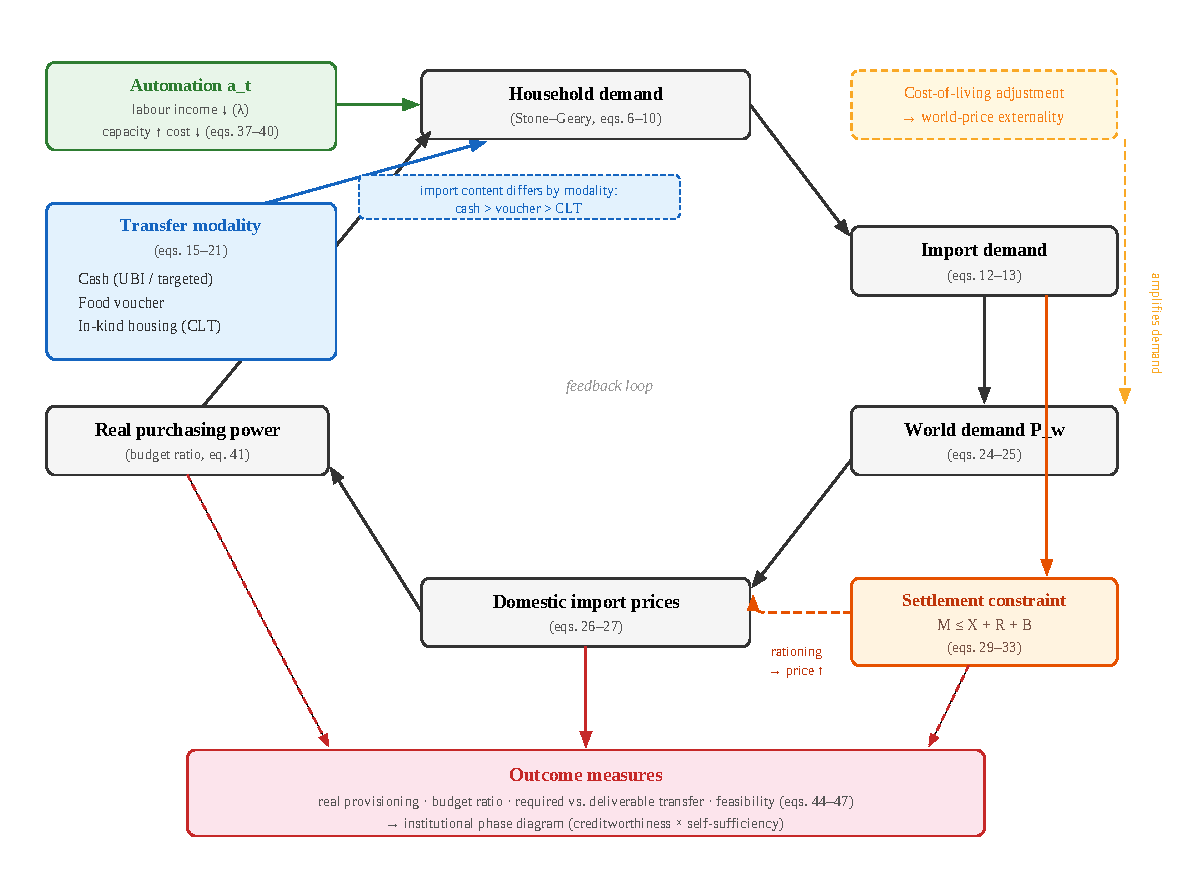
\includegraphics[width=\textwidth]{figure1_schematic.pdf}
\caption{Model architecture. Solid arrows trace the central feedback loop: household demand generates import demand, which feeds world demand pressure, which raises domestic import prices, which reduces real purchasing power, which feeds back to household demand. The settlement constraint (orange) rations imports when foreign-exchange resources are insufficient, raising prices further. Transfer modality (blue) enters through household demand; the import content of spending differs by modality. Automation (green) reduces labour income and raises capacity simultaneously. Cost-of-living adjustment (dashed yellow) amplifies world demand pressure through a cumulative externality. Outcome measures (red) aggregate the loop into feasibility criteria and the institutional phase diagram.}
\label{fig:schematic}
\end{figure}

Automation enters from above: a single automation path reduces labour
income and shifts it toward capital, while simultaneously raising
potential productive capacity and lowering unit costs. The model thus
has two parallel series --- a baseline without automation and a
post-employment transition with automation at various levels --- that
share the same structure and differ only in the ceiling of this path.

Three closed-world accounting identities hold at every period: the sum
of all current accounts equals zero, the sum of all capital accounts
equals zero, and the sum of all changes in net foreign assets equals
zero. Writing \(X_{it}\) for export earnings, \(M_{it}\) for imports,
\(CA_{it} = X_{it} - M_{it}\) for the current account, \(K_{it}\) for
the net capital flow, and \(\mathrm{NFA}_{it}\) for net foreign assets,

\[\sum_i CA_{it} = 0, \qquad \sum_i K_{it} = 0, \qquad \sum_i \Delta \mathrm{NFA}_{it} = \sum_i \left( CA_{it} + K_{it} \right) = 0. \tag{1}\]

The identities hold to a tolerance of \(10^{-10}\) (Appendix A).\footnote{The
model tracks foreign-exchange reserves \(R_{it}\) (equation 33) rather than a
full balance sheet of gross foreign assets and liabilities. The closure
identity (1) holds on net flows; what it verifies is that the system is
closed --- no spending leaks out --- not that each bloc's gross asset and
liability positions are individually reconciled.} No spending leaks out
of the system. A bloc's import is another bloc's
export revenue. A bloc's capital outflow is another bloc's inflow. This
closure is a deliberate methodological choice: it ensures that the
advantage or disadvantage of any transfer modality cannot arise from
spending that disappears at the border.

\subsection{Economic blocs and international accounting}

The world is divided into blocs positioned on a two-dimensional plane.
The horizontal axis is creditworthiness: a bloc's capacity to borrow in
international markets, determined by its credit standing, debt ratio,
and risk premium. The vertical axis is self-sufficiency: the domestic
content of what the bloc consumes, with food as its defining component.
Four archetypes anchor the corners of this plane: a reserve-currency
bloc with high creditworthiness and high self-sufficiency, an advanced
bloc with high creditworthiness and lower self-sufficiency, an emerging
bloc with moderate creditworthiness and moderate self-sufficiency, and a
developing bloc with low creditworthiness and low self-sufficiency. A
grid of twenty-five blocs populates the plane, with creditworthiness and
self-sufficiency varying independently across five levels each.

Each bloc occupies a position \((c_i, \psi_i) \in [0,1]^2\), with
\(c_i, \psi_i \in \{0, 0.25, 0.5, 0.75, 1\}\), and every structural
parameter \(\vartheta\) attached to an axis is interpolated linearly
between that axis's endpoints:

\[\vartheta_i = \vartheta^{\mathrm{lo}} + \left( \vartheta^{\mathrm{hi}} - \vartheta^{\mathrm{lo}} \right) \cdot \mathrm{position}_i. \tag{2}\]

Along the creditworthiness axis, from worst to best, the policy rate
runs from 0.070 to 0.020, the baseline foreign-asset share of saving
from 0.35 to 0.05, credit standing \(\varsigma_i\) from 0.15 to 1.6, and
opening reserve standing from 0.25 to 1.75; the foreign-currency share
of debt is \(f_i = 0.85\,(1 - c_i)\). Along the self-sufficiency axis,
the import contents of food, general goods, and construction run from
\((m^F, m^G, m^H) = (0.30, 0.35, 0.25)\) to \((0.10, 0.15, 0.05)\). The
reserve issuer sits at \((1, 1)\).

This two-dimensional parameterisation replaces the simpler four-bloc
structure used in early phases of the model. Its purpose is to separate
two mechanisms that prior work has conflated: the inability to borrow (a
creditworthiness problem) and the inability to produce what is consumed
(a self-sufficiency problem). A bloc with low creditworthiness but high
self-sufficiency faces a different constraint from a bloc with high
creditworthiness but low self-sufficiency. The former cannot borrow but
does not need to import much; the latter can borrow but accumulates debt
as imports grow. The phase diagram that constitutes the paper's main
result depends on this separation.

Each bloc is further described by an initial GDP and debt ratio, trade
openness \(o_i\), a trend growth rate, and a constrained household block
(Section 3.3); Table B.2 lists the archetype values. A bloc's exports
are the imports of the other blocs, distributed by supplier shares that
depend on economic size, openness, and --- when the trade elasticity
\(\epsilon_T\) is active --- the supplier's exchange rate:

\[\begin{gathered} S_{ij} = \frac{v_j \, e_{jt}^{\,\epsilon_T}}{\sum_{k \neq i} v_k \, e_{kt}^{\,\epsilon_T}} \;\; (j \neq i), \\ S_{ii} = 0, \\ v_i = Y_{i0} \, o_i, \\ X_{jt} = \sum_i S_{ij} M_{it}. \end{gathered} \tag{3}\]

Because each row of \(S\) sums to one, \(\sum_i X_{it} = \sum_i M_{it}\)
holds by construction. The world supply capacity grows along a path
calibrated to the realised traded-goods demand of the no-transfer
baseline (Section 3.5), ensuring that the model's supply side does not
embed an assumption about the secular trend.

\subsection{Household demand}

Households within each bloc are divided into two groups: constrained
households, whose income is at or below the level needed to meet
subsistence requirements, and unconstrained households, whose income
exceeds subsistence. The constrained block is a share \(n_i\) of the
population receiving a share \(\sigma_i\) of output; both are structural
parameters of each bloc, fixed for the duration of the simulation. What
changes endogenously is the constrained group's real income, which
responds to labour income, transfers, prices, and exchange-rate
movements. Its income is

\[I^c_{it} = \sigma_i \, Y_{it} \, \phi^{\mathrm{inc}}_{it} \, \lambda_t, \tag{4}\]

where \(Y_{it}\) is bloc output, \(\lambda_t\) is the automation
labour-income multiplier (Section 3.7), and \(\phi^{\mathrm{inc}}_{it}\)
is an income-linkage factor: \(\phi^{\mathrm{inc}}_{it} = 1\) when
constrained income keeps pace with output, \(Y_{i0}/Y_{it}\) when it
holds its opening real value, and \(Y_{i0}/(Y_{it}\,\Pi_{it})\) when it
is fixed in nominal terms, with \(\Pi_{it}\) the bloc's price level. The
post-employment series uses the second rule. Within the constrained
block, income can be divided into \(k\) equal-population quantiles with
different income weights and subsistence tilts (equation B.1); the
post-employment series uses five.

Only the constrained block's household problem is solved. The
unconstrained block enters through the increment of income that reaches
it,

\[\Delta I^u_{it} = \mathrm{cash}^u_{it} + \Delta \mathrm{rent}_{it} + D_{it}, \tag{5}\]

where \(\mathrm{cash}^u_{it}\) is its share of any universal payment
together with land payments under the CLT, \(\Delta \mathrm{rent}_{it}\)
is the change in rent income, and \(D_{it}\) is labour income displaced
by automation, which accrues to the owners of the machines (equation
38). The unconstrained block spends a fraction \(\mathrm{mpc}^u = 0.3\)
of this increment. Because its own consumption problem is never solved,
aggregate provisioning and aggregate demand cannot be summed across the
two blocks.

Constrained households allocate spending through a linear expenditure
system (LES) derived from Stone--Geary preferences. Each household has
subsistence requirements for food (measured in physical units), housing
(measured in floor area), and general consumption:

\[\bar{x}^k_{it} = \gamma^k \, I^c_{it}, \qquad (\gamma^F, \gamma^G, \gamma^H) = (0.35,\, 0.05,\, 0.25). \tag{6}\]

The requirement is a quantity set in proportion to the group's current
income; it does not respond to prices. The basic-needs bundle used to
measure affordability (Section 3.8) is defined separately and held fixed
in physical terms throughout the run. Spending above subsistence is
allocated across the three categories according to marginal budget
shares \(\beta^k\). Let \(M\) be cash income available for market
purchases and \(f^k\) the quantity of good \(k\) received in kind (zero
unless a voucher or CLT programme is running). Full income and
supernumerary income are

\[\tilde{M} = M + \sum_k p^k f^k, \qquad \Omega = \tilde{M} - \sum_k p^k \bar{x}^k, \tag{7}\]

and the interior allocation is

\[x^k = \bar{x}^k + \frac{\beta^k \max(\Omega, 0)}{p^k}, \qquad (\beta^F, \beta^G, \beta^H) = (0.25,\, 0.45,\, 0.30). \tag{8}\]

The key property of this demand system is that the subsistence
requirement does not shrink when prices rise, so that price increases
tighten the budget rather than reducing consumption proportionally. The
model does not represent an allocation below subsistence, where
Stone--Geary utility is undefined; the bound at zero in (8) is an
implementation measure, not a behavioural claim. Where the constraint
binds, the reported demand quantity \(x^k\) may exceed what the
household can actually purchase. This is conservative for the paper's
central finding: it overstates real provisioning in precisely the
positions where cash transfers perform worst, so the feasibility
boundary reported for cash regimes is, if anything, too generous.

When an in-kind grant exceeds what the household would freely choose,
that good's quantity is pinned at the grant and the remaining budget is
reallocated. With binding set \(\mathcal{J} = \{k : x^k < f^k\}\) and
its complement \(\mathcal{J}^c\),

\[\begin{gathered} x^k = f^k \;\; (k \in \mathcal{J}), \\ x^k = \bar{x}^k + \frac{\beta^k}{\sum_{j \in \mathcal{J}^c} \beta^j} \cdot \frac{\max(\Omega', 0)}{p^k} \;\; (k \in \mathcal{J}^c), \\ \Omega' = M + \sum_{k \notin \mathcal{J}} p^k f^k - \sum_{k \in \mathcal{J}^c} p^k \bar{x}^k. \end{gathered} \tag{9}\]

This is what makes an inframarginal in-kind grant equivalent to cash and
an extramarginal one not. Market expenditure and utility are

\[b^k = p^k \max\left(0,\; x^k - f^k\right), \qquad U = \sum_k \beta^k \ln\left(x^k - \bar{x}^k\right), \tag{10}\]

with \(U = -10^9\) assigned when any \(x^k \le \bar{x}^k\).

Housing rent is not given by a formula but clears the rental market.
Rental supply is anchored so that the no-transfer economy clears at
\(p^H = 1\), and the rent \(p^H_{it}\) solves

\[\begin{gathered} \frac{b^H(p^H)}{p^H} = S^0_i \, (p^H)^{\varepsilon_i \mu}, \\ S^0_i = \bar{x}^H + \beta^H \left( I^c_i - \bar{x}^F - \bar{x}^G - \bar{x}^H \right), \end{gathered} \tag{11}\]

where \(\varepsilon_i\) is the short-run rental supply elasticity and
\(\mu\) a uniform multiplier on it.

The import content of spending differs across categories. Food has an
import content \(m^F_i\) set by the bloc's position on the
self-sufficiency axis, from 0.30 at its low end to 0.10 at its high end.
General consumption has a separate, higher import content \(m^G_i\).
Housing spending is largely domestic --- construction labour and land
are non-traded --- but building materials carry an import content
\(m^H_i\). Imports are carried in two measures that are not
interchangeable --- spending, which enters the balance of payments, and
quantity, which enters the world market:

\[M^{\mathrm{sp}}_{it} = m^F_i \, b^F_{it} + m^G_i \, b^G_{it}, \qquad M^{\mathrm{q}}_{it} = m^F_i \, x^F_{it} + m^G_i \, x^G_{it}. \tag{12}\]

Import demand facing the world is the no-programme level plus the
increment the programme causes,

\[\begin{gathered} M_{it} = M^{\mathrm{sp},0}_{it} + \Delta M_{it}, \\ \Delta M_{it} = \left( M^{\mathrm{sp},1}_{it} - M^{\mathrm{sp},0}_{it} \right) + M^{\mathrm{gov}}_{it} + \mathrm{mpc}^u \, m^G_i \, \Delta I^u_{it}, \end{gathered} \tag{13}\]

where superscripts 0 and 1 denote household demand solved without and
with the programme, and \(M^{\mathrm{gov}}_{it}\) is the import content
of government procurement for in-kind programmes (equation B.3). It is
the level, not the increment, that must clear the world market;
otherwise a world-wide programme would appear as demand against zero
capacity. These import contents translate household demand into
foreign-exchange requirements, which is the channel through which the
transfer modality affects the settlement constraint.

The constrained block does not save. The unconstrained block saves the
fraction \(1 - \mathrm{mpc}^u\) of the increment that reaches it and
places a share \(\omega_{it}\) of that saving abroad through a
behavioural rule: the foreign-asset share responds to the risk premium
\(rp_{it}\) (Section 3.6) and to recent exchange-rate depreciation,

\[\begin{gathered} \omega_{it} = \min\left( 0.9,\; \max\left( 0,\; \omega^0_i + \nu_\omega \left( rp_{it} + \max\left(0, \dot{e}_{it}/\Delta\right) \right) \right) \right), \\ FA_{it} = \left( 1 - \mathrm{mpc}^u \right) \Delta I^u_{it} \, \omega_{it} \, o_i, \end{gathered} \tag{14}\]

where \(\omega^0_i\) is the bloc's baseline foreign-asset share,
\(\nu_\omega = 2.0\), and \(\dot{e}_{it}\) is last period's change in
the exchange rate. Foreign-asset purchases are a capital outflow, not a
purchase of goods: they enter the capital account, not world demand for
tradables. This is a reduced-form specification, not an intertemporal
optimisation. Section 5 demonstrates that the main results are robust to
variation in the parameters of this rule. The sensitivity analysis
sweeps the capital-inflow-to-demand parameter from zero to one and shows
that the gap between modalities widens rather than closes, confirming
that the results do not depend on the specific portfolio closure.

\subsection{Transfer modalities and welfare equivalence}

The model implements four redistributive policy regimes, which differ
along two dimensions: targeting (universal versus means-tested) and
modality (cash versus in-kind).

Each programme has a size \(u_i\), expressed as a share of GDP. Its
budget is a share of current real output when no indexation rule is in
force, and a nominal amount \(T_{it}\) carried across periods under an
indexation rule (equation 22):

\[\mathcal{B}_{it} = \begin{cases} u_i \, Y_{it} & \text{no indexation rule} \\ T_{it} & \text{under an indexation rule.} \end{cases} \tag{15}\]

Universal cash (UBI) pays out the whole budget, split between the
constrained and unconstrained blocks by population share. Targeted cash
directs the whole budget to constrained households only, so the
per-recipient amount is higher:

\[\begin{aligned} &\text{UBI:} && T^{\mathrm{cash},c}_{it} = \mathcal{B}_{it} \, n_i, && T^{\mathrm{cash},u}_{it} = \mathcal{B}_{it} (1 - n_i), \\ &\text{targeted:} && T^{\mathrm{cash},c}_{it} = \mathcal{B}_{it}, && T^{\mathrm{cash},u}_{it} = 0, \end{aligned} \qquad F_{it} = \mathcal{B}_{it}, \tag{16}\]

where \(F_{it}\) is the programme's fiscal cost. Food vouchers provide a
means-tested entitlement that can be spent only on food; unused portions
do not convert to cash, which is the extramarginal case of (9). The
grant enters demand as a quantity of food,

\[f^F_{it} = \begin{cases} u_i \, Y_{it} & \text{no indexation rule} \\ \mathcal{B}_{it} / p^F_{it} & \text{under an indexation rule,} \end{cases} \qquad F_{it} = p^F_{it} \, f^F_{it}, \tag{17}\]

so that under an indexation rule what the budget buys falls as food
becomes dearer. In-kind housing provides a physical dwelling ---
represented as a community land trust (CLT) unit --- that removes the
housing cost of the granted unit from the recipient's budget; housing
consumed beyond the grant is bought at the market rent, by (10). The
land beneath the dwelling is held in trust and does not enter the
market. The grant enters demand as a quantity of floor area,

\[f^H_{it} = \begin{cases} u_i \, Y_{it} & \text{no indexation rule} \\ \mathcal{B}_{it} & \text{under an indexation rule.} \end{cases} \tag{18}\]

Unlike the voucher, the CLT quantity is not divided by a price: once
built, the units stay built. Equation (18) specifies the per-period
grant; the cumulative housing stock available to recipients is limited
by a finite build rate (equation B.4).

The comparison between universal cash and targeted cash isolates the
effect of targeting. The comparison among targeted cash, food vouchers,
and in-kind housing --- all means-tested --- isolates the effect of
transfer modality holding targeting constant. Results that differ
between targeted cash and in-kind housing are therefore attributable to
modality, not to the breadth of coverage.

The CLT is treated as a representative case of non-fugitive in-kind
asset provisioning, not as a faithful reproduction of any specific CLT
programme. Its defining properties for the model are three: land enters
the transfer cost at an acquisition discount rather than at market rent,
it has lower import content than a cash transfer of equivalent welfare
value (because housing services are largely non-traded), and its real
value does not depreciate with the exchange rate (because the dwelling
exists physically regardless of currency movements). The fiscal cost of
in-kind housing splits into structure and land:

\[\begin{gathered} C^{\mathrm{build}}_{it} = (1 - \ell_i) \, f^H_{it} \, (1 + \kappa_s h_i), \\ C^{\mathrm{land}}_{it} = \ell_i \, (1 - \delta_L) \, \frac{r_{it} + 0.02}{r_{i0} + 0.02} \, f^H_{it}, \\ F_{it} = C^{\mathrm{build}}_{it} + C^{\mathrm{land}}_{it}, \end{gathered} \tag{19}\]

where \(\ell_i\) is land's share of gross rent, \(\delta_L = 0.5\) the
acquisition discount, \(r_{i0}\) the pre-transfer interest rate, \(h_i\)
the policy effort to source construction domestically, and \(\kappa_s\)
the cost markup that such sourcing carries, local supply being thinner
than the import market. The land payment accrues to landowners and
enters \(\mathrm{cash}^u_{it}\) in (5). Because rent is a flow and
construction a stock, the rent the trust collects on its own units is
credited against the programme's cost after annualisation at the bloc's
own cost of capital over the building's life of \(n_L = 40\) years:

\[\begin{gathered} A(r_i, n_L) = \frac{r_i}{1 - (1 + r_i)^{-n_L}}, \\ R^{\mathrm{CLT}}_{it} = \mathcal{R}_{it} \cdot \frac{f^H_{it}}{S^0_i \, (p^H_{it})^{\varepsilon_i \mu} + f^H_{it}} \cdot A(r_i, n_L), \end{gathered} \tag{20}\]

with \(A = 1/n_L\) when \(r_i = 0\), and \(\mathcal{R}_{it}\) the rent
flow in the housing market. A high-rate bloc therefore amortises faster,
and the annualised fiscal burden is not a one-time expenditure compared
against ongoing cash flows. A finite build rate can phase the programme
in (equation B.4). The model does not represent housing quality,
locational choice, spatial concentration, or governance costs, all of
which would affect the real-world viability of such provision. These
omissions are stated as limitations.

All four modalities are calibrated to deliver the same level of
household welfare at the moment of introduction. This welfare-equivalent
calibration is essential to the paper's argument: the comparison is not
between a generous programme and a stingy one but between programmes
that start from the same objective and diverge through their
macrofinancial dynamics. The calibration takes as its target the
constrained household's Stone--Geary utility (10) under UBI of size
\(u\), evaluated at introduction prices (\(Y_i\) at its opening value,
\(e_i = 1\)), and finds for each other modality the size that reaches
it:

\[\begin{gathered} U^\star_i = U_i(\mathrm{ubi},\, u), \\ u^{\mathrm{mod}}_i = \left\{ u' : U_i(\mathrm{mod},\, u') = U^\star_i \right\}, \\ \mathrm{mod} \in \{\text{targeted cash, voucher, CLT}\}, \end{gathered} \tag{21}\]

solved by bisection on \(u' \in [0, 0.5]\). The search returns a bound
rather than a solution in two cases --- when it converges below the
target utility, and when the required size reaches the ceiling of 0.5 of
GDP --- and whether either occurs in a reported run is a result, not a
given. An equal-cost calibration, which instead equates the fiscal cost
\(F_i/Y_i\) across modalities, is also available.

Each transfer is subject to a policy rule governing its nominal value
over time. Under cost-of-living adjustment, the nominal transfer is
increased each quarter by the quarterly fraction of the previous
period's annual consumer-price inflation, preserving the transfer's
purchasing power with a one-period lag. Under nominal freeze, the
transfer amount is fixed at its initial value and erodes as prices rise.
A third rule, used where indexation is not the object of comparison,
keeps the transfer at a fixed share of current real output:

\[T_{it} = \begin{cases} T_{i,t-1} \left( 1 + \pi_{i,t-1} \Delta \right) & \text{cost-of-living adjustment} \\ T_{i,t^{\mathrm{start}}} & \text{nominal freeze} \\ u_i \, Y_{it} & \text{output-linked,} \end{cases} \qquad T_{i,t^{\mathrm{start}}} = u_i \, Y_{i,t^{\mathrm{start}}}. \tag{22}\]

Indexing to the previous period's inflation reflects the lag in real
indexation arrangements and keeps the transfer and the inflation it
causes from becoming simultaneous. The transfer's real value relative to
its opening value is

\[\mathrm{RV}_{it} = \frac{T_{it} / \Pi_{it}}{T_{i,t^{\mathrm{start}}} / \Pi_{i,t^{\mathrm{start}}}}, \tag{23}\]

with an analogous measure in terms of rent (equation B.5), which shows
that a transfer can hold its value in consumption goods while losing it
in housing. The first two rules define the horns of a dilemma that the
results section documents: adjustment protects recipients but raises
fiscal costs and generates a world-price externality; freezing avoids
the externality but abandons recipients to inflation.

\subsection{World market and price formation}

All blocs' import demands aggregate into a single world traded-goods
market. The demand-pressure variable, denoted \(P_w\), is an index of
the extent to which aggregate traded-goods demand exceeds aggregate
supply capacity. It is a model-internal intermediate variable, not a
quantity that corresponds to any observable real-world aggregate. Its
role is mechanical: it transmits the aggregate demand pressure into each
bloc's import price through the exchange rate. With \(Z_t\) the world's
traded-goods supply capacity, the gap is excess world demand as a
fraction of capacity, and the index evolves in logs with a slow
reversion to a fixed anchor \(P_{w,0} = 1\):

\[g_t = \frac{\sum_i M^{\mathrm{q}}_{it}}{Z_t} - 1, \tag{24}\]

\[\begin{gathered} \hat{\pi}^w_t = \kappa_w \, g_t - \lambda_w \ln\left( \frac{P_{w,t}}{P_{w,0}} \right), \\ P_{w,t+1} = \min\left( \bar{P},\; \max\left( 10^{-6},\; P_{w,t} \exp\left[ \min\left( \hat{\pi}^w_t \Delta,\; 20 \right) \right] \right) \right), \end{gathered} \tag{25}\]

with \(\kappa_w = 0.35\) and \(\lambda_w = 0.05\). The reversion is
taken in logs because a restoring term written on the level grows
without bound and can drive the index negative. The anchor does not
drift, so a transitory gap does not shift the level permanently, while a
sustained gap still moves it without limit. The cap
\(\bar{P} = 10^{12}\) is a reporting limit: a configuration that reaches
it is one whose indexation loop ran away.

Each bloc's import price is the index converted at its exchange rate
\(e_{it}\) and marked up by the scarcity \(s_{it}\) left from last
period's rationing (Section 3.6). Domestic components cost one by
normalisation, scaled by the automation unit-cost multiplier \(c_t\)
(Section 3.7). Food and general-goods prices are weighted averages of
the two:

\[\tau_{it} = \frac{e_{it} \, P_{w,t}}{\max\left( 10^{-6},\; 1 - \min(0.95,\, s_{it}) \right)}, \tag{26}\]

\[p^F_{it} = \left[ (1 - m^F_i) \, c_t + m^F_i \, \tau_{it} \right] \varphi_{it}, \qquad p^G_{it} = (1 - m^G_i) \, c_t + m^G_i \, \tau_{it}, \tag{27}\]

where \(\varphi_{it}\) is a food-price shock multiplier equal to one in
the main series. Without scarcity and without a food shock, the food
price is \(p^F_{it} = (1 - m^F_i)\,c_t + m^F_i \, e_{it} P_{w,t}\),
where \(m^F_i\) is the food import content and \(e_{it}\) is the nominal
exchange rate. A bloc with high self-sufficiency (low \(m^F_i\)) is
insulated from movements in \(P_w\); a bloc with low self-sufficiency is
exposed. This is the channel through which one bloc's transfer spending
--- by contributing to aggregate traded-goods demand --- raises another
bloc's food prices. Rationing reaches what a household eats in the same
way, as a price: a bloc rationed to part of its import demand faces a
traded-goods price high enough to clear the quantity it can pay for.
Bloc inflation responds to the change in import prices, to the domestic
demand pull of the programme, and to a central-bank drag (equation B.7).

The supply capacity of the world grows at a rate calibrated to the
no-transfer baseline's realised traded-goods demand, so that the model's
supply side does not build in inflationary or deflationary bias. Opening
capacity is normalised on the first period's no-transfer demand, so that
the baseline opens at a zero gap, and capacity growth is weighted by
demand:

\[\begin{gathered} Z_0 = \sum_i M^{\mathrm{q}}_{i0}, \\ \hat{g}^Z_t = \frac{\sum_i M^{\mathrm{q}}_{it} \max\left( 0.005,\; g^{\mathrm{base}}_i - \delta_i t \right)}{\sum_i M^{\mathrm{q}}_{it}}, \end{gathered} \tag{28}\]

where \(g^{\mathrm{base}}_i\) is the bloc's trend growth and
\(\delta_i\) its annual decline. The path is fixed once from a
no-transfer run, iterated to a fixed point with realised demand, and
shared by every configuration, so that a programme's demand cannot call
forth the supply to meet it. Under the post-employment transition,
automation raises potential capacity, but actual output is
demand-constrained: excess capacity drags on the growth rate rather than
being produced and left unsold (Section 3.7).

\subsection{International settlement and monetary hierarchy}

Each non-reserve bloc faces a settlement constraint: its imports in any
period cannot exceed the sum of its export earnings \(X_{it}\), its
foreign-exchange reserves \(R_{it}\), and the amount \(B_{it}\) it can
borrow on international markets:

\[\begin{gathered} \mathcal{K}_{it} = \max\left( 0,\; X_{it} + R_{it} + B_{it} \right), \\ M^{\mathrm{real}}_{it} = \min\left( M_{it},\; \mathcal{K}_{it} \right). \end{gathered} \tag{29}\]

Borrowing capacity is a function of the bloc's credit standing
\(\varsigma_i\), which is reduced by the contagion state \(\chi_{it}\),
and of the risk premium, which rises with the debt ratio \(d_{it}\),
inflation, and foreign-currency exposure:

\[\begin{gathered} \varsigma_{it} = \varsigma_i \max\left( 0,\; 1 - \chi_{it} \right), \\ B_{it} = \max\left( 0,\; Y_{it} \, \bar{b} \, \Delta \, \varsigma_{it} \max\left( 0,\; 1 - \nu_b \, rp_{it} \right) \right), \end{gathered} \tag{30}\]

\[rp_{it} = \kappa_r \max(0,\, d_{it} - \bar{d}) + \tfrac{\kappa_r}{2} \max(0,\, \pi_{it} - 0.06) + \tfrac{\kappa_r}{2} f_i \max(0,\, d_{it} - 0.6) + \kappa_c \, \chi_{it}, \tag{31}\]

with \(\bar{b} = 0.05\) per year, \(\nu_b = 4\), \(\kappa_r = 0.15\),
\(\bar{d} = 0.9\), and \(\kappa_c = 0.05\); at a premium of \(1/\nu_b\)
the borrowing window shuts. Credit standing is kept separate from the
opening debt level: giving a low-credit bloc a low opening debt would
make its premium small and its borrowing window wide, inverting the
axis. When the constraint binds, imports are rationed --- the bloc
receives less than its households demand --- and in the following period
domestic prices rise to reflect the scarcity, through (26):

\[\begin{gathered} \mathrm{Rationed}_{it} = \max\left( 0,\; M_{it} - M^{\mathrm{real}}_{it} \right), \\ s_{i,t+1} = \frac{\mathrm{Rationed}_{it}}{M_{it}}, \\ M^{\mathrm{q,real}}_{it} = M^{\mathrm{q}}_{it} \, \frac{M^{\mathrm{real}}_{it}}{M_{it}}, \end{gathered} \tag{32}\]

with \(s_{i,t+1} = 0\) when \(M_{it} = 0\). Rationing is applied before
the world re-clears, because one bloc's cut imports remove another
bloc's exports. Reserves evolve as

\[R_{i,t+1} = \max\left( 0,\; R_{it} + X_{it} - M^{\mathrm{real}}_{it} + K_{it} \Delta \right). \tag{33}\]

Here \(K_{it}\) is the net capital flow as in (1), not the settlement
capacity \(\mathcal{K}_{it}\) of (29). The exchange rate responds to
capital flows and to the demand for foreign exchange --- the current account less the unsettled shortfall,
so that a bloc rationed because its reserves ran out is not read as
strengthening --- with a response proportional to the current rate
rather than additive (equation B.6).

The reserve-currency bloc settles in money it issues: while it holds
that position, its imports are not rationed and
\(M^{\mathrm{real}}_{it} = M_{it}\). Reserve-currency status is
represented as an institutional difference in settlement capacity ---
the issuing bloc's import payments do not draw down a finite stock of
foreign exchange --- rather than through ad hoc preferential
coefficients applied to risk premia, capital flows, or exchange-rate
adjustment. The position lasts only as long as other blocs want to hold
the currency. Reserves are held to settle future imports, so their
attraction is what they will buy:

\[\begin{gathered} \mathcal{D}_t = \mathcal{D}_0 \left( \frac{1}{P_{w,t}} \right)^{\epsilon_R}, \\ \mathcal{D}_0 = \sum_{i \,:\, \neg \mathrm{reserve}} Y_{i0} \, o_i, \\ \mathrm{exempt}_{it} = \mathrm{reserve}_i \wedge \neg\left[ \mathcal{D}_t < \bar{\theta}_R \, \mathcal{D}_0 \right], \end{gathered} \tag{34}\]

with \(\epsilon_R = 0.5\) and \(\bar{\theta}_R = 0.7\), both swept
rather than chosen. Conditional advantages then emerge endogenously from
the resulting trade, price, and contagion dynamics. At low transfer
levels, the reserve bloc's position on the
creditworthiness--self-sufficiency plane naturally protects it: its
distance from blocs that experience settlement failure is large, and
contagion does not reach it. As the transfer level rises toward
\(u \approx 0.055\), this protection disappears --- not because the
model withdraws a privilege but because the number and proximity of
distressed blocs increase until the reserve bloc is no longer distant
from all of them.

Financial contagion operates through a similarity channel rather than
through direct financial linkages. When a bloc experiences settlement
failure, lenders reassess blocs with similar structural characteristics
--- a wake-up-call mechanism (Ahnert and Bertsch, 2022). When bloc \(j\)
defaults, every other bloc's contagion state is raised according to its
structural distance from \(j\), measured by credit standing and food
import content, and the shock decays geometrically over \(Y_c = 5\)
years:

\[\begin{gathered} \mathrm{dist}(i,j) = \sqrt{ \left( \frac{|\varsigma_i - \varsigma_j|}{1.6} \right)^2 + \left( \frac{|m^F_i - m^F_j|}{0.25} \right)^2 }, \\ \chi_{it} \leftarrow \min\left( 1,\; \chi_{it} + \varkappa \, e^{-\mathrm{dist}(i,j)/\varrho} \right), \\ \chi_{i,t+1} = \chi_{it} \left( 1 - \frac{\Delta}{Y_c} \right), \end{gathered} \tag{35}\]

with reach \(\varrho = 0.5\) and strength \(\varkappa\). Because the
grid moves the three import contents together, distance in \(m^F\) is
monotone in position on the self-sufficiency axis. The contagion state
raises the risk premium (31) and cuts effective credit standing (30), so
the reassessment raises risk premia and tightens borrowing capacity for
blocs that are structurally proximate to the failed bloc. The reserve
issuer is not exempted by assertion; a flight-to-reserve channel routes
the withdrawn funds to it as a consequence (equation B.9). This produces
a contagion pattern that is ordered by structural position rather than
by trade volume or financial exposure.

Policy response is modelled as a reduced-form reaction to gaps relative
to the world. A bloc whose growth falls short of the size-weighted world
rate \(\hat{g}^W_t\), or whose real interest rate falls short of the
world yardstick \(\bar{r}^W_t\), receives an impulse split between a
policy-rate cut and a fiscal boost:

\[\begin{gathered} \mathrm{gap}_{it} = \max\left( 0,\; \hat{g}^W_t - \hat{g}_{it} \right) + \max\left( 0,\; \bar{r}^W_t - (r_{it} - \pi_{it}) \right), \\ \mathrm{cut}_{it} = \kappa_P \, \mathrm{gap}_{it} \, (1 - \varphi_F), \\ \mathrm{boost}_{it} = \kappa_P \, \mathrm{gap}_{it} \, \varphi_F, \end{gathered} \tag{36}\]

with \(\varphi_F = 0.5\). The rule is identical in every bloc and names
no target. The adjustment faces a dilemma: easing depreciates the
exchange rate and tightens the settlement constraint; tightening slows
growth and induces capital outflow that depletes reserves. The results
show that outcomes do not improve monotonically with the strength of the
policy response.

\subsection{Post-employment transition}

The post-employment transition is driven by automation progress \(a_t\),
which approaches a ceiling \(a_{\max}\) exponentially, so that the early
years move fastest and the last of the work is hardest to automate:

\[a_t = a_{\max} \left( 1 - e^{-\nu_a t} \right), \qquad \nu_a = 0.15 \text{ per year}. \tag{37}\]

From this single path, four consequences are derived simultaneously:

\[\begin{gathered} \Lambda_t = 1 + \alpha_K \, a_t, \qquad c_t = \max\left( 0.05,\; 1 - \alpha_C \, a_t \right), \\ \lambda_t = \max\left( 0,\; 1 - \alpha_L \, a_t \right), \qquad D_{it} = \sigma_i \, Y_{it} \left( 1 - \lambda_t \right), \end{gathered} \tag{38}\]

with \(\alpha_K = 1.0\), \(\alpha_C = 0.3\), and \(\alpha_L = 1.0\).
Potential productive capacity rises by the factor \(\Lambda_t\), unit
costs fall by the factor \(c_t\), the constrained block's labour income
is multiplied by \(\lambda_t\) in (4) --- so that labour's share of
income falls as a consequence --- and the income that labour loses,
\(D_{it}\), shifts to capital, entering the unconstrained block through
(5). Note that \(D_{it} = \sigma_i Y_{it}(1 - \lambda_t)\) measures
the economy-wide shift from labour income to capital income within the
constrained sector's output share. It is not identical to the change
in the constrained block's received income, which also depends on the
income-linkage factor \(\phi^{\mathrm{inc}}_{it}\) in (4). These four effects are not independently calibrated --- they are
joint consequences of the same technological change, which is the
defining feature of a post-employment transition as distinct from a
sectoral productivity shock.

Potential output carries the bloc's realised trend
\(Y^{\mathrm{trend}}_{it}\) (equation B.8) multiplied by the automation
factor, and the shortfall of output below potential drags on the growth
rate:

\[\begin{gathered} Y^{\mathrm{pot}}_{it} = Y^{\mathrm{trend}}_{it} \, \Lambda_t, \\ \mathrm{slack}_{it} = \max\left( 0,\; 1 - \frac{Y_{it}}{Y^{\mathrm{pot}}_{it}} \right), \end{gathered} \tag{39}\]

\[\begin{gathered} \hat{g}_{it} = g^{\mathrm{eff}}_{it} + 0.08 \, \eta_f \, \frac{\Delta \mathrm{Dom}_{it}}{Y_{it}} - \alpha_D \, \mathrm{slack}_{it} + \textstyle\sum \mathrm{penalties}_{it}, \\ Y_{i,t+1} = \max\left( 0.01,\; Y_{it} \left( 1 + \hat{g}_{it} \Delta \right) \right), \end{gathered} \tag{40}\]

where
\(g^{\mathrm{eff}}_{it} = \max(0.005,\, g^{\mathrm{base}}_i - \delta_i t)\)
is trend growth, \(\Delta \mathrm{Dom}_{it}\) the change in domestic
demand the programme causes (equation B.2), \(\eta_f = 1.2\) a fiscal
multiplier, and the penalties are reduced-form terms for capital flows,
debt, inflation, and exchange-rate movement (equation B.8). The
parameter \(\alpha_D\) sets how strongly the demand shortfall holds
output down and is swept; at \(\alpha_D = 0\) output follows trend
growth plus the fiscal impulse regardless of whether what is made can be
bought. Output is not capped at potential. When automation raises
potential capacity but labour income falls, a gap opens between what the
economy could produce and what households can buy, and the resulting
slack drags on the growth rate through (40). Transfers fill this gap
partially, but the transfer itself generates import demand that
encounters the settlement constraint. The question the model answers is
whether the transfer can fill the gap before the settlement constraint
closes it --- and for which blocs, under which policy regime, this is
possible.

The model runs two parallel series: a baseline with \(a_{\max} = 0\), in
which no automation occurs, and a post-employment series with
\(a_{\max}\) at 0.2, 0.4, 0.6, or 0.8. The baseline establishes the
benchmark against which the post-employment results are evaluated.

\subsection{Outcome measures and feasibility criterion}

The model reports outcomes in real physical quantities rather than in
monetary aggregates. The primary measure is real provisioning: the
quantity of housing (floor area) and food (caloric equivalent) that
transfer recipients actually secure in each period. This is the only
metric that places cash and in-kind transfers on a common footing --- a
cash transfer that depreciates before it is spent delivers less
provisioning than its nominal value suggests.

The budget ratio is defined as the ratio of a constrained household's
total resources (income plus transfer) to the cost of a fixed
basic-needs bundle, where the bundle is defined in physical quantities
(a specified amount of food, housing, and general consumption at current
prices). For income quantile \(q\) of the constrained block, with income
share \(\varpi_q\) and population share \(n_q\),

\[\begin{gathered} \mathrm{BR}_{iqt} = \frac{I_{iqt} + T_{iqt}}{\sum_k p^k_{it} \, \hat{x}^k_{iq}}, \\ I_{iqt} = \sigma_i \, Y_{it} \, \phi^{\mathrm{inc}}_{it} \, \lambda_t \, \varpi_q, \\ T_{iqt} = T_{it} \, n_q. \end{gathered} \tag{41}\]

The bundle quantities are fixed once, at a reference income
\(I^{c,\mathrm{ref}}_i\), and do not move; only prices do:

\[\hat{x}^k_{iq} = \gamma^k \, I^{c,\mathrm{ref}}_i \, \theta \, \zeta_q, \tag{42}\]

where \(\theta\) scales the floor and \(\zeta_q\) is the quantile's
subsistence tilt (equation B.1). A budget ratio below one means the
household cannot afford the bundle. The ratio says whether the money
reaches the bundle, not whether the household is fed.

The required transfer level, \(u^\star\), is the transfer as a share of
GDP that closes the largest quantile shortfall relative to that
quantile's population share. With a single constrained type this is the
whole constrained block; under the five-quantile configuration of the
post-employment series it is the quantile with the largest gap, which
need not be the poorest by income. Because the ratio is linear in the
transfer, the requirement at given prices is solved directly:

\[\begin{gathered} T^\star_{it} = \frac{1}{\max\left( 0.05,\; \mathrm{RV}_{it} \right)} \max_q \left[ \frac{\max\left( 0,\; \sum_k p^k_{it} \hat{x}^k_{iq} - I_{iqt} \right)}{n_q} \right], \\ u^\star_{it} = \frac{T^\star_{it}}{Y_{it}}. \end{gathered} \tag{43}\]

The divisor \(\mathrm{RV}_{it}\) from (23) puts the indexation rules on
a common footing: a transfer that has lost half its real value must have
been twice as large to begin with. The requirement is a time series, not
a constant: as the currency falls and the demand-pressure index rises,
the bundle costs more, and the blocs where it grows fastest are those
least able to pay. For the fixed point below, the requirement is taken
as its maximum over the run's sampled years.

Because the transfer itself changes prices, exchange rates, and import
costs, \(u^\star\) is not a simple arithmetic calculation but a fixed
point: the transfer level at which the budget ratio equals one, taking
into account all the equilibrium adjustments that the transfer induces.
The model searches for this fixed point on a discrete candidate grid
\(\mathcal{U} = \{0, 0.01, 0.02, 0.03, 0.04, 0.06, 0.08, 0.12\}\) for at
most six rounds:

\[\begin{gathered} u^{(0)} = u^\star_i \big|_{u=0}, \\ u^{(n+1)} = \min\left\{ u \in \mathcal{U} : u \ge u^\star_i \big|_{u = u^{(n)}} \right\}, \\ u^{\mathrm{FP}}_i = u^{(n+1)} \;\; \text{if} \;\; u^\star_i \big|_{u = u^{(n+1)}} \le u^{(n+1)}. \end{gathered} \tag{44}\]

The fixed point is therefore grid-valued, and ``no fixed point'' means
that none was found on this grid within six rounds.

The deliverable transfer level is the largest candidate whose average
rationing share over the run stays within a tolerance \(\varepsilon\):

\[\begin{gathered} \bar{s}_i \big|_u = \frac{1}{N_s} \sum_t s_{it} \big|_u, \\ u^{\mathrm{del}}_i(\varepsilon) = \max\left\{ u \in \mathcal{U} : \bar{s}_i \big|_u \le \varepsilon \right\}, \\ \varepsilon \in \{0,\, 0.05,\, 0.10\}. \end{gathered} \tag{45}\]

When the required level exceeds the deliverable level, the bloc is in a
provisioning trap: it cannot deliver what its population needs without
exhausting its capacity to import.

Each bloc is classified at each automation level by four conditions:

\[\begin{aligned}
&\textbf{already constrained:} && \bar{s}_i \big|_{u=0} > 10^{-12}, \\
&\textbf{no fixed point:} && u^{\mathrm{FP}}_i \text{ undefined} \;\wedge\; u^\star_i \big|_{u=0} > 0, \\
&\textbf{trapped}(\varepsilon): && u^\star_i \big|_{u=0} > 0 \;\wedge\; \bar{s}_i \big|_{u=0} \le 10^{-12} \\ &&& \wedge\; \left( u^{\mathrm{FP}}_i \text{ undefined} \;\vee\; u^{\mathrm{del}}_i(\varepsilon) \text{ undefined} \;\vee\; u^{\mathrm{FP}}_i > u^{\mathrm{del}}_i(\varepsilon) \right), \\
&\textbf{feasible:} && \text{none of the above.}
\end{aligned} \tag{46}\]

A bloc is already constrained when its imports are rationed even without
any transfer. The four conditions are evaluated independently and are
not mutually exclusive; the classification applies them in order of
precedence --- already constrained, no fixed point, trapped, feasible.
The no-fixed-point state, which emerges at high automation levels, means
that every additional unit of transfer raises prices and import costs
enough to require more than one additional unit --- the system diverges.

Crisis outcomes are reported as continuous excess measures rather than
as a single crisis count. For each bloc, the debt ratio, inflation, and
the exchange rate are compared with reporting cut-offs of 1.5, 0.15, and
2.0:

\[\begin{gathered} \mathrm{exc}_{it} = \left( \frac{\max(0,\, d_{it} - 1.5)}{1.5},\; \frac{\max(0,\, \pi_{it} - 0.15)}{0.15},\; \frac{\max(0,\, e_{it} - 2.0)}{2.0} \right), \\ \mathrm{severity}_i = \sum_t \Big( \sum \mathrm{exc}_{it} \Big) \Delta, \\ \mathrm{duration}_i = \sum_t \mathbb{1}\left[ \mathrm{exc}_{it} \neq 0 \right]. \end{gathered} \tag{47}\]

Onsets are counted on transitions into crisis, and insolvency is
recorded when the debt ratio exceeds 3.0, after which the bloc's state
stops being updated. The cut-offs are reporting thresholds, not
structural boundaries. Outcomes are thus reported along five dimensions
--- onset, duration, severity, insolvency year, and breadth (number of
blocs simultaneously in crisis) --- rather than as a single crisis
count. This decomposition addresses a specific criticism of an earlier
version of the model. World-level pressure is reported as levels and
changes of the demand-pressure index, the world gap, and the share of
demand coming from solvent blocs, with no verdict threshold (equation
B.12); imports and foreign-asset purchases are reported separately,
because only the first buys goods on the world market (equation B.13).

\section{Results}

Results are presented in five stages, ordered by the logic of the
argument rather than by the sequence in which the model was constructed.

\subsection{Same welfare, different macroeconomic footprints}

When all four policy regimes are calibrated to deliver the same welfare
gain to constrained households at the moment of introduction, they
produce sharply different macroeconomic consequences over a thirty-year
horizon. Table 1 reports the key indicators for a representative
low-creditworthiness, low-self-sufficiency bloc (the developing
archetype) under the baseline scenario with cost-of-living adjustment.

\begin{table}[htbp]
\centering
\caption{Welfare-equivalent comparison at year 30, developing bloc,
baseline with cost-of-living adjustment ($u = 0.02$, all blocs
introducing simultaneously). Fiscal scale is the outlay at introduction.
Import demand is cumulative real imports over the run, indexed to the
no-transfer run. Depreciation is the exchange rate at year 30 against its
year-1 value. Food and housing are the physical quantities secured by
constrained households, each indexed to its own run's year 1. The budget
ratio is the poorest quantile's income plus transfer over the cost of the
fixed subsistence bundle. The settlement constraint is inactive in this
configuration; Sections 4.3 and 4.5 report what happens when it binds.}
\label{tab:same-welfare}
\setlength{\tabcolsep}{5pt}
\begin{tabular}{lcccccc}
\hline
         & Fiscal  & Import  & Depre-   &        &         & Budget \\
Modality & scale   & demand  & ciation  & Food   & Housing & ratio  \\
         & (\% GDP) & index  & (\%)     & (phys.) & (phys.) & (Q1)   \\
\hline
UBI                  & 2.0 & 93.1  & $+234$ & 149.7 & 136.7 & 1.710 \\
Targeted cash        & 1.0 & 99.8  & $+128$ & 180.9 & 190.1 & 2.230 \\
Food voucher         & 1.0 & 101.1 & $+156$ & 170.8 & 175.6 & 2.016 \\
In-kind housing      & 0.4 & 101.5 & $+89$  & 188.7 & 198.9 & 2.254 \\
\hline
\textit{No transfer} & 0.0 & 100.0 & $+77$  & 191.3 & 197.4 & 2.184 \\
\hline
\end{tabular}
\end{table}

Three patterns are visible. First, the required fiscal scale differs
across modalities even though the initial welfare objective is
identical. Universal cash requires the largest outlay because the
payment goes to all households; targeted cash is smaller because it
reaches only constrained households; in-kind housing is smaller still
because it removes the housing component from the monetary transfer and
replaces it with a physical asset whose cost does not include land rent.
Second, the import demand generated by each modality differs because the
spending composition differs. Cash transfers are spent according to
household preferences, which in a low-self-sufficiency bloc means a
large fraction goes to imported food and goods. Housing provision
generates demand primarily for construction labour and materials, of
which the import share is lower. Third, and most strikingly, in-kind
housing improves food provisioning despite distributing no food. The
mechanism is indirect: by removing rent from the household budget,
housing provision frees income for food spending. At year thirty, the
developing bloc's constrained households secure housing quantities
approximately equal to the no-transfer baseline (198.9 versus 197.4 on
the year-1 index), while under universal cash the same households secure
only 136.7 --- less than they would have had with no transfer at all. The
same ordering holds for food (188.7 for in-kind housing, 149.7 for
universal cash, against 191.3 with no transfer).

This last result deserves emphasis. It means that in the developing
archetype, a universal cash transfer calibrated to improve welfare at
introduction makes recipients materially worse off over a thirty-year
horizon than doing nothing. The transfer's macrofinancial consequences
--- exchange-rate depreciation and import-price increases caused by the
aggregate demand it generates --- take away more than the transfer
gives. This is not a theoretical curiosity; it is a transfer reversal
--- a state in which the transfer itself becomes the proximate cause of
welfare deterioration. It differs from the provisioning trap defined in
Section 3.8, where the required transfer level exists but exceeds what
the settlement constraint can deliver. Here the transfer is delivered,
but the price it sets in motion undoes its benefit.

\subsection{Transmission mechanism decomposition}

The divergence between modalities operates through a chain of
transmission that can be decomposed into distinct steps. The chain runs
as follows: the transfer modality determines the fiscal scale; the
fiscal scale and spending composition determine sectoral demand;
sectoral demand determines import demand; import demand contributes to
world traded-goods demand pressure; the demand-pressure index feeds
through exchange rates into each bloc's import prices; import prices
determine the real purchasing power of the transfer; and real purchasing
power determines the provisioning that households actually secure.

At each step, the modalities diverge further. Universal cash generates
the highest fiscal outlay, the largest exchange-rate depreciation (+234
percent over thirty years, against +77 percent with no transfer at all),
the largest import-price increase, and therefore the smallest real
provisioning. In-kind housing generates the smallest fiscal outlay in
monetary terms, the least depreciation (+89 percent), and therefore the
largest real provisioning.

The import column of Table 1 does not follow that ordering, and the
reason is worth stating because it is easy to misread. Universal cash
generates the \emph{lowest} cumulative real imports of the four (93.1
against the no-transfer run's 100.0), below in-kind housing's 101.5,
while depreciating the currency three times as far. This is not because
universal cash asks less of the world market: its marginal import leak is
in fact the largest of the four modalities (0.40 against in-kind housing's
0.19, in the units of Appendix B.3). It is because the depreciation it
sets off makes imports expensive enough that the realised quantity ends
up below what the same bloc would have bought with no programme at all.
The level of imports and the pressure that produced it are therefore not
the same measurement, and it is the price, not the quantity, that decides
what households secure.

Food vouchers, despite being means-tested, concentrate all spending into
a single category --- food --- so their import demand per unit of
welfare can exceed that of universal cash, even though general goods
carry a higher import content per unit of spending (\(m^G_i > m^F_i\)). This is why vouchers produce
more fixed-point failures than universal cash at automation 0.4 (Section
4.4): the constraint is not the total fiscal outlay but the import
composition of spending.

A second distinction runs through the capital account rather than the
current account. Universal cash is the only regime that pays the
unconstrained block (equation 16): the share \((1 - n_i)\) of the budget
that reaches unconstrained households enters the saving channel and,
through the foreign-asset allocation rule (equation 14), generates
capital outflows that deplete reserves and depreciate the exchange rate.
Targeted cash, vouchers, and in-kind housing direct the full budget to
constrained households, who do not save in the model. The capital-flight
channel is therefore UBI-specific. Vouchers and targeted cash cannot
leak through the capital account at all --- but vouchers concentrate
their entire demand on imported food, while UBI spreads demand across
categories and loses part of its budget to capital outflow rather than
goods demand. The net effect is that UBI's capital-account leak,
paradoxically, reduces its current-account pressure relative to a
voucher of equivalent welfare: the money that flees the country does not
buy imported food.

There is a second, independent channel that operates only for housing
provision. When a CLT supplies housing directly, the market rent that
constrained households would otherwise have paid is removed from the
demand side of the housing market. This does not raise the supply of
housing in the market (the CLT units are additional), but it does reduce
the competition for market-rate housing among unconstrained households,
exerting modest downward pressure on market rents. The freed budget ---
income that would have gone to rent --- is redirected to food and
general consumption. This is why housing provision improves food
outcomes: it is not a food programme, but it loosens the budget
constraint in the direction of food.

The decomposition also explains why universal cash makes recipients in
the developing archetype worse off than no transfer. The transfer adds
to the household's income, but that income is spent in an economy with
high import dependence. The currency depreciates by 234 percent over
thirty years, against 77 percent in the same bloc with no transfer at
all, and the resulting rise in import prices affects all households,
including the transfer recipients themselves. When the indirect induced
penalties --- all channels removed from the model except exchange-rate
and import-price effects --- are eliminated, seventy-nine to eighty-five
percent of the shortfall against the no-transfer baseline remains. The damage is not driven by
behavioural penalties or stigma effects but by the macrofinancial
arithmetic of settlement.

\subsection{Monetary hierarchy and heterogeneous feasibility}

The twenty-five-bloc plane reveals that different structural positions
produce different kinds of failure, and that the type of failure --- not
just its occurrence --- depends on the two axes independently.

Insolvency is primarily structured by creditworthiness. Blocs with low
creditworthiness exhaust their borrowing capacity first, because they
begin with lower reserves, face higher risk premia, and have smaller
stocks of net foreign assets to draw down. A bloc at creditworthiness
level one reaches settlement failure earlier and at lower transfer
levels than a bloc at level three, holding self-sufficiency constant.
This is the channel through which original sin operates in the model:
the inability to borrow is the proximate cause of import rationing.

Import compression is primarily structured by self-sufficiency. Blocs
with low self-sufficiency need more imports for the same level of
provisioning, so they draw down reserves faster and hit the settlement
constraint sooner. But a surprising interaction emerges: blocs with high
self-sufficiency are partially protected even at low creditworthiness.
Because they import less, their current-account deficits are smaller,
debt accumulates more slowly, and the settlement constraint binds later
or not at all. At self-sufficiency 0.892, a bloc at the lowest
creditworthiness level avoids insolvency entirely at moderate transfer
levels, whereas the same creditworthiness at self-sufficiency 0.689
produces insolvency within fifteen years.

The reserve-currency bloc's protection is conditional. At low transfer
levels (u = 0.04), it receives a contagion exposure of 0.477 while all
other blocs receive 1.000 --- a protection that arises purely from its
distance on the two-axis plane from the blocs that experience failure.
At u $\approx$ 0.055, this protection disappears: enough blocs have failed, and
the surviving blocs are close enough to the reserve bloc on at least one
axis, that the wake-up-call contagion reaches it. The boundary is not a
crisis count but a geometric property of the distribution of failures on
the plane.

Policy response offers no escape for blocs at structurally disadvantaged
positions. Monetary easing depreciates the exchange rate, which tightens
the settlement constraint by raising the domestic-currency cost of
imports. Monetary tightening slows growth, which induces capital
outflows that deplete reserves. The result is non-monotonic: outcomes
for blocs with low creditworthiness and low self-sufficiency do not
improve continuously with the strength of the policy response.

\subsection{Post-employment transition shrinks the feasible set}

Under the baseline scenario (no automation), provisioning traps appear
only when three conditions are met simultaneously: no compression of
consumption below subsistence is tolerated, the basic-needs floor
exceeds seventy-five percent of the reference level, and the transfer is
not adjusted for inflation. Remove any one condition and the trap
disappears.

When automation is introduced, all three conditions become unnecessary.
At automation level 0.4, traps appear even when moderate consumption
compression is tolerated. At 0.6, traps appear even at a basic-needs
floor of fifty percent. At 0.4 and above, traps appear whether or not
the transfer is adjusted for inflation --- though nominal freeze
produces more trapped positions (nineteen) than cost-of-living
adjustment (eight) at automation 0.4.

The required transfer level rises steeply with automation. At automation
0.8, the required transfer to maintain the poorest quintile's budget
ratio at one reaches approximately 9.6 percent of GDP. The deliverable
transfer --- the maximum that can be sustained without triggering
settlement failure --- is approximately 8.0 percent of GDP under a
tolerance of ten percent import rationing. Because the required level
exceeds the deliverable level, these blocs are in a provisioning trap:
the fixed point u* exists on the candidate grid but lies outside the
feasible range. At still higher automation levels, a distinct and more
severe state emerges: no candidate on the grid \(\mathcal{U}\) achieves
\(B(u) \geq 1\) within six rounds --- every additional unit of transfer
raises prices and import costs by more than one unit, and the solver
does not converge.

At automation 0.4, the four regimes separate sharply. Of the twenty-five
positions, six are already constrained (rationed with no transfer).
Among the remaining nineteen, in-kind housing retains feasibility at all
nineteen positions with no fixed-point failures. Targeted cash is
feasible at sixteen positions with three fixed-point failures. Universal
cash is feasible at twelve with seven failures. Food vouchers are
feasible at only nine with ten failures --- worse than universal cash,
because the voucher's extramarginal constraint channels all spending
into food imports, concentrating import demand in the category with the
highest price sensitivity. The ordering of regimes by feasibility is
therefore not a simple cash-versus-in-kind ranking: CLT dominates,
followed by targeted cash, then universal cash, then vouchers. But even
in-kind housing eventually loses feasibility at the highest automation
levels for the most structurally disadvantaged positions.

\subsection{Cost-of-living adjustment externality and coordination failure}

Cost-of-living adjustment of transfers --- increasing the nominal
payment each period by the previous period's consumer-price inflation
--- generates a world-price externality that has not, to our knowledge,
previously been shown in simulation.

The mechanism is straightforward. An adjusted transfer tracks prices
upward, which maintains the recipient's purchasing power but also
maintains the recipient's demand for traded goods. That demand
contributes to world traded-goods demand pressure, which raises import
prices for all blocs, which raises consumer prices, which triggers a
further adjustment. The loop does not explode --- each iteration is
damped by the one-period lag and by the domestic production share ---
but over thirty years it produces a cumulative difference.

When all twenty-four non-reserve blocs adjust their transfers and the
counterfactual is that none adjust, six to nine of those blocs
experience worse budget ratios than they would have had without
adjustment. A representative low-creditworthiness, low-self-sufficiency
bloc illustrates the mechanism: the real value of its transfer is 0.40
units higher than under nominal freeze (the adjustment works), but its
budget ratio is 0.13 lower (the import-price increase caused by
everyone's adjustment more than offsets the gain). The remaining blocs
see smaller losses that do not reverse the sign of the budget-ratio
change but do reduce the gain from adjustment. The collectively
rational decision --- refrain from adjustment --- is undermined by the
individually rational incentive to adjust, because nominal freeze
guarantees erosion of the real transfer value.

This is a world-price externality with the structure of a coordination
problem. Each bloc's adjustment maintains its own demand for traded
goods, which contributes to world demand pressure, which raises import
prices for all blocs. The food export-restriction literature documents
an analogous mechanism: each country that restricts exports to insulate
its domestic food price raises the world price that all other countries
face (Martin and Anderson, 2012). Confirming that non-adjustment is
individually unsustainable --- that a single bloc freezing its transfer
while others adjust is made worse off --- would require a one-bloc
deviation experiment that is not part of the present design, which
models only world-wide simultaneous adoption.

\subsection{Institutional feasibility phase diagram}

\begin{figure}[htbp]
\centering
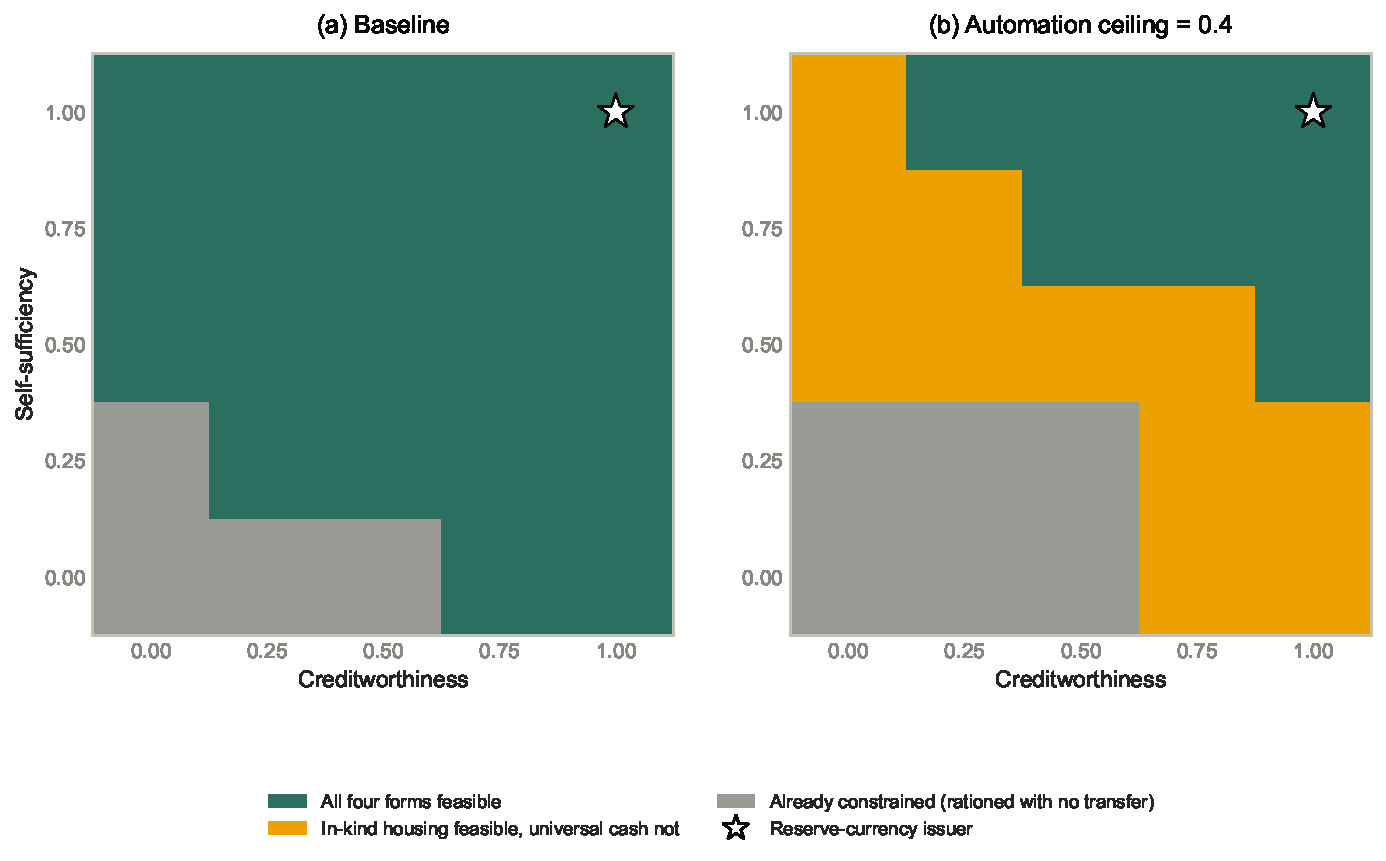
\includegraphics[width=\textwidth]{figure2_phase_diagram.pdf}
\caption{Institutional feasibility by creditworthiness and self-sufficiency. Each cell is one of 25 blocs. Colour shows the set of policy regimes that remain feasible over 30 years. Under automation (b), the feasible frontier shifts inward and the regimes separate. Positions already rationed with no transfer at all are shown separately, because there the constraint is not a statement about what is handed out. A fourth state --- no form feasible --- is defined but occurs at no position in either panel, and is therefore absent from the legend.}
\label{fig:phase-diagram}
\end{figure}


The phase diagram --- the paper's culminating result --- displays the
interaction between structural position, transfer modality, and
automation visually. Two panels show the twenty-five positions on the
creditworthiness--self-sufficiency plane, one for the baseline and one
for automation at 0.4. Each position is coloured by the set of policy
regimes that remain feasible. Under the baseline, the feasible sets are
nearly identical across regimes: all four regimes are feasible at every
position that is not already constrained. Under automation 0.4, the sets
separate. In-kind housing retains feasibility at every non-constrained
position. The cash regimes and the voucher lose feasibility at positions
with low creditworthiness or low self-sufficiency, but at different
rates and in a pattern that is not simply ordered by the two axes: at
(0.00, 0.75), universal cash is feasible but targeted cash shows no
fixed point, because the higher per-recipient amount under targeting
concentrates demand pressure. The boundary between feasible and
infeasible shifts inward --- toward higher creditworthiness and higher
self-sufficiency --- for all regimes except in-kind housing. The figure
shows that the international monetary system does not merely limit how
much redistribution a country can afford. It selects which institutional
forms of redistribution can survive.

\section{Robustness}

The main results --- the divergence of macrofinancial footprints across
modalities, the phase-diagram structure, and the shrinkage of feasible
sets under automation --- are tested against variation in the model's
key assumptions. Full sensitivity tables are reported in Supplementary
Material; this section summarises the findings.

Portfolio and capital-flow closure. The foreign-asset allocation rule is
behavioural rather than derived from intertemporal optimisation. To
assess sensitivity to one key aspect of this specification, the
capital-inflow-to-demand parameter --- which governs how much of capital
inflows translates into real goods demand --- is swept from zero (no
pass-through) to one (full pass-through). The gap between policy regimes
widens as the parameter increases: at zero, the traded-goods
demand-pressure index under universal cash is 1.465 and under in-kind
housing is 1.158; at 0.5, the corresponding values are 4.255 and 1.390.
The widening occurs because capital inflows under cash transfers amplify
domestic demand, which feeds back into imports and exchange-rate
pressure. The result confirms that the main findings are robust to
alternative assumptions about the real-demand pass-through of capital
inflows and, if anything, are conservative under the baseline
specification. A full sweep of the portfolio-allocation parameters ($\omega_0$,
$\omega_s$) is reported in Supplementary Material.

Cost-of-living adjustment rules. Three rules are compared: full
adjustment to previous-period CPI, partial adjustment (fifty percent of
CPI growth), and nominal freeze. Full adjustment produces fewer
provisioning traps than nominal freeze at all automation levels, but the
world-price externality is larger. Partial adjustment lies between the
two. The qualitative structure of the phase diagram ---
modality-dependent feasible sets ordered by structural position --- is
invariant across rules.

Subsistence floor. The basic-needs floor is varied from fifty to one
hundred percent of the reference level in increments of five percentage
points. At fifty percent, provisioning traps under the baseline
disappear entirely. At seventy-five percent, traps appear only when all
three baseline conditions are met. At one hundred percent (no
compression tolerated), traps appear more widely. Under automation at
0.4 or above, traps appear at every floor level, confirming that the
post-employment result does not depend on the choice of subsistence
threshold.

Contagion strength. The wake-up-call contagion parameter is varied from
zero (no contagion) to twice the baseline value. Without contagion, the
number of blocs experiencing settlement failure is lower, but the
phase-diagram structure persists because the primary driver is each
bloc's own settlement arithmetic. Stronger contagion accelerates failure
for structurally proximate blocs and shifts the reserve-currency bloc's
protection boundary to lower transfer levels. The qualitative ordering
of modalities is unchanged.

Transfer level. The transfer is swept from zero to twelve percent of
GDP. The divergence between modalities is small at low transfer levels
and grows monotonically. Below two percent of GDP, all four modalities
produce similar outcomes because the macrofinancial footprint is small
relative to the economy. Above five percent, the separation becomes
pronounced. This confirms that the results are about large-scale
redistribution, not about marginal transfers.

World supply elasticity. When the world supply capacity responds more
elastically to demand, the demand-pressure effect is dampened and the
gap between modalities narrows. When supply is inelastic --- as it would
be under physical capacity constraints or during a supply-chain
disruption --- the gap widens. The results are sensitive to this
parameter in magnitude but not in sign or structure.

Housing and CLT construction assumptions. The import content of housing
construction is varied from ten to forty percent. At higher import
content, the advantage of in-kind housing narrows because more of its
cost generates foreign-exchange demand. At forty percent import content,
in-kind housing still dominates cash in the developing archetype, but
the margin is reduced by approximately half. This confirms that the
advantage of housing provision depends in part on the non-traded
character of construction, which varies across countries.

\begin{center}\rule{0.5\linewidth}{0.5pt}\end{center}

\section{Discussion}

\subsection{Redistribution as institutional design}

The central finding of this paper is that welfare-equivalent transfers
can produce radically different macrofinancial outcomes. This means that
the question ``how much redistribution can a country afford?'' is
incomplete without the companion question ``in what institutional
form?'' The fiscal cost of a transfer is one dimension of its
feasibility; its import content, its exposure to exchange-rate
movements, and its contribution to world demand pressure are others. A
country that can afford a cash transfer in domestic-budget terms may be
unable to sustain it in settlement terms, while the same welfare
objective delivered through in-kind asset provision may remain feasible.

This is not a new insight in the abstract --- the humanitarian
literature has long recognised that market conditions affect the choice
between cash and in-kind aid --- but to our knowledge the present paper
provides the first formal model in which the institutional form of
redistribution interacts with international monetary constraints to
determine feasibility. The result generalises beyond the specific
modalities modelled here: any transfer whose spending composition
generates high import demand will face tighter settlement constraints
than one whose composition is more domestically oriented, holding the
welfare objective constant.

\subsection{Monetary hierarchy as institutional selection}

The phase diagram shows that the international monetary system does not
merely limit the quantity of redistribution. It selects which
institutional forms of redistribution can survive at each structural
position. A country with low creditworthiness and low food
self-sufficiency faces a smaller set of viable redistributive
institutions than a country with high creditworthiness and high
self-sufficiency. The reserve-currency country faces the largest set,
but even its feasible set contracts as the transfer level rises.

This selection pressure is structural, not deliberate. No agent in the
model designs the monetary hierarchy to favour one form of
redistribution over another. The selection arises from the arithmetic of
settlement: different policy regimes generate different import demands,
which encounter different settlement capacities, which produce different
real outcomes.

The world-price externality documented in Section 4.5 adds a
collective-action dimension to this selection. When all countries
simultaneously adjust their transfers for inflation, the aggregate
effect raises world traded-goods demand and import prices for all
countries, including the adjusting countries themselves. Six to nine of
twenty-four non-reserve blocs end up with worse budget ratios than they
would have had without adjustment; the remaining blocs see their gains
from adjustment reduced. Whether non-adjustment is individually
sustainable --- whether a single country that freezes its transfer while
others adjust is made worse off --- remains untested in the present
design, which models only world-wide simultaneous adoption (Section
4.5). The externality is structurally analogous to the food
export-restriction externality documented by Martin and Anderson (2012),
in which each country's price-insulation policy raises the world price
that all other countries face.

\subsection{Post-employment amplification}

Under the baseline scenario, the selection pressure is visible only at
the margins of the creditworthiness--self-sufficiency plane. Most
positions can sustain all four regimes. The post-employment transition
amplifies the selection pressure by simultaneously raising the required
transfer level (because labour income falls) and tightening the
settlement constraint (because the transfer generates more import demand
than the shrinking labour income can finance through exports). At
automation 0.4, the feasible sets diverge: in-kind housing retains
feasibility at every non-constrained position, while universal cash and
food vouchers lose it at seven and ten positions respectively. At higher
automation levels, even in-kind housing loses feasibility at the most
structurally disadvantaged positions.

This amplification justifies the paper's title and framing. The
post-employment transition is not a speculative scenario appended to the
model for completeness; it is the condition under which the model's
central findings become practically relevant. Under the baseline, the
institutional form of redistribution is a design choice with moderate
macrofinancial consequences. Under post-employment, it becomes a binding
constraint that determines whether provisioning is possible at all.

\subsection{The exit direction: self-sufficiency is not fixed}

The model treats food self-sufficiency as structural over the simulation
horizon, but it is a policy variable over longer horizons. The
provisioning trap depends on food import dependence, and food import
dependence can be moved. Historical evidence demonstrates that locally
optimised, ecologically embedded intensive agriculture can achieve high
per-unit productivity while absorbing large quantities of labour:
Mesoamerican chinampa agriculture produced thirteen times the output of
dry-land farming, and Andean terrace systems sustained millions without
market exchange (Sophia, 2026). The inverse farm-size--yield
relationship, established since Sen (1962, 1966) and robust below
approximately three to five hectares (Muyanga and Jayne, 2019), provides
the modern empirical foundation. The strongest counterargument ---
Foster and Rosenzweig's (2022) estimate that consolidating farms to
optimal scale would raise income per worker by sixty-eight percent ---
assumes that displaced agricultural labour is absorbed by the non-farm
sector. Under post-employment conditions, that assumption fails
(Chiarella, Meyfroidt, Abeygunawardane, and Conforti, 2023). Investments
in food-system resilience and import-substituting productive capacity
may therefore shift a bloc upward on the phase diagram, but this
transition requires low dependence on imported inputs, as Sri Lanka's
2022 experience demonstrates (FAO and WFP, 2022). Modelling that
transition is left for future work.

\begin{center}\rule{0.5\linewidth}{0.5pt}\end{center}

\section{Limitations}

The model is a computational exploration, not a calibrated forecasting
tool. Several limitations constrain the interpretation of its results.

Household portfolio allocation is represented by a behavioural rule
rather than derived from intertemporal optimisation. The sensitivity
analysis in Section 5 shows that the main results are robust to
variation in this rule, but the model cannot speak to the dynamics of
portfolio rebalancing under uncertainty.

The economic blocs are stylised archetypes positioned on a
two-dimensional plane, not calibrated representations of specific
national economies. The results identify structural patterns --- which
positions are vulnerable to which failures under which modalities ---
but do not predict outcomes for any named country.

The model does not include a banking sector. Credit creation, interbank
lending, and the amplification of shocks through bank balance sheets are
absent. In a world where financial crises often originate in the banking
sector, this is a significant omission.

Political adaptation beyond the modelled policy response is not
represented. Governments in practice adjust fiscal and monetary policy
in complex ways that depend on political constraints, institutional
capacity, and public pressure. The reduced-form policy response captures
the qualitative dilemma (easing versus tightening) but not the full
range of political responses.

Post-collapse dynamics are not modelled. The paper's motivation --- that
government failure can lead to civil disorder, armed conflict, and
refugee flows --- is precisely the set of outcomes that the model does
not represent. The model identifies the economic conditions under which
provisioning fails; what follows from that failure is outside its scope.

Within-bloc household heterogeneity is limited to the
constrained/unconstrained division and to income quantiles within the
constrained block; the unconstrained block's consumption problem is not
solved. The model does not represent urban--rural differences, regional
variation, or occupational structure within a bloc.

The automation pathway is stylised. Automation progress follows a fixed
exponential path toward its ceiling, and its consequences are derived
from a single structural relationship. The model does not estimate the
speed, sectoral incidence, or upper bound of automation.

Housing quality, locational choice, and spatial concentration are not
modelled. In-kind housing provision in the model delivers a homogeneous
unit of floor area. In practice, publicly provided housing varies
enormously in quality and location, and concentrated provision can
produce spatial segregation and stigma. These costs may be substantial
and would reduce the advantage of in-kind provision relative to cash.

The basic-needs level is not calibrated to any empirical standard.
Results are reported as response surfaces across a range of floor
levels, so the reader can assess the sensitivity, but the model does not
claim to identify a specific subsistence threshold.

Each bloc's position on the creditworthiness--self-sufficiency plane is
fixed for the duration of the simulation. In practice, a bloc that
invested in domestic food production or in export capacity could move to
a less constrained position over time. Modelling such transitions would
require specifying an investment pathway whose speed, cost, and
political feasibility are not predictable from the model's structure;
the phase diagram should therefore be read as showing which positions
are vulnerable under current structural conditions, not as a permanent
sentence.

The subsistence floor that enters household choice (equation 6) is
proportional to current income, whereas the bundle used to measure
affordability (equation 42) is fixed in physical quantities. The two are
deliberately different --- a floor proportional to income cannot fall
short, because if income halves so does the floor --- but they are not
the same object, and results on the budget ratio refer to the fixed
bundle.

\begin{center}\rule{0.5\linewidth}{0.5pt}\end{center}

\section{Conclusion}

This paper asked whether every country can sustain the provisioning of
its population when labour income falls simultaneously across the world
economy. The answer is that it depends on what form the provisioning
takes and where the country stands in the international monetary
hierarchy.

A multi-bloc computational model with closed-world accounting,
foreign-exchange settlement constraints, and welfare-equivalent
calibration shows that transfer modalities that are identical in their
immediate welfare gain produce radically different macrofinancial
trajectories. Cash transfers generate high import demand, depreciate the
exchange rate, and raise domestic prices through the traded-goods
channel; in structurally disadvantaged positions --- low
creditworthiness, low food self-sufficiency --- they make recipients
worse off than no transfer at all. In-kind asset provisioning reduces
import content, excludes land rent from the transfer cost, and preserves
real value through exchange-rate movements, retaining feasibility at
positions where cash has failed. Post-employment transition amplifies
this divergence: as automation raises the required transfer level, the
feasible set of institutions contracts, and the modalities separate.
Cost-of-living adjustment of transfers, individually rational, generates
a world-price externality that collectively undermines the provisioning
it was designed to protect.

The implication extends beyond the specific modalities and parameters
examined here. Open-economy constraints do not merely limit the quantity
of redistribution that a country can afford. They shape the
institutional forms through which redistribution remains economically
feasible. The international monetary system, through the arithmetic of
settlement, exerts a selection pressure on redistributive institutions
--- a pressure that intensifies as the need for redistribution grows.
The design of redistribution is therefore not only a question of
domestic political economy but an international structural problem whose
solution requires attention to the form of provisioning, not only its
scale.

\begin{center}\rule{0.5\linewidth}{0.5pt}\end{center}




\section*{Declaration of generative AI and AI-assisted technologies in the writing process} During the preparation of this work the author used Claude (Anthropic) to assist with simulation code development, literature search, equation extraction from code, and manuscript drafting. The author reviewed and edited all AI-generated content and takes full responsibility for the content of the publication.
\begin{thebibliography}{99} 
\bibitem{Acemoglu2018} Acemoglu, D., \& Restrepo, P. (2018). \emph{Artificial intelligence, automation, and work} (NBER Working Paper No.~24196). National Bureau of Economic Research. https://doi.org/10.3386/w24196 
\bibitem{Ahnert2022} Ahnert, T., \& Bertsch, C. (2022). A wake-up call theory of contagion. \emph{Review of Finance, 26}(4), 829--854. https://doi.org/10.1093/rof/rfac025 
\bibitem{Alonso2022} Alonso, C., Berg, A., Kothari, S., Papageorgiou, C., \& Rehman, S. (2022). Will the AI revolution cause a great divergence? \emph{Journal of Monetary Economics, 127}, 18--37. https://doi.org/10.1016/j.jmoneco.2022.01.004 
\bibitem{Autor2015} Autor, D. H. (2015). Why are there still so many jobs? The history and future of workplace automation. \emph{Journal of Economic Perspectives, 29}(3), 3--30. https://doi.org/10.1257/jep.29.3.3 
\bibitem{Banerjee2019} Banerjee, A., Niehaus, P., \& Suri, T. (2019). Universal basic income in the developing world. \emph{Annual Review of Economics, 11}, 959--983. https://doi.org/10.1146/annurev-economics-080218-030229 
\bibitem{Bonizzi2019} Bonizzi, B., Kaltenbrunner, A., \& Michell, J. (2019). Monetary sovereignty is a spectrum: Modern monetary theory and developing countries. \emph{Real-World Economics Review, 89}, 46--61. 
\bibitem{Bourassa2007} Bourassa, S. C. (2007). Community land trusts and housing affordability. In G. K. Ingram \& Y.-H. Hong (Eds.), \emph{Land policies and their outcomes} (pp.~333--366). Lincoln Institute of Land Policy. 
\bibitem{Chahrour2022} Chahrour, R., \& Valchev, R. (2022). Trade finance and the durability of the dollar. \emph{Review of Economic Studies, 89}(4), 1873--1910. https://doi.org/10.1093/restud/rdab072 
\bibitem{Chenery1966} Chenery, H. B., \& Strout, A. M. (1966). Foreign assistance and economic development. \emph{American Economic Review, 56}(4), 679--733. 
\bibitem{Chiarella2023} Chiarella, C., Meyfroidt, P., Abeygunawardane, D., \& Conforti, P. (2023). Balancing the trade-offs between land productivity, labor productivity and labor intensity. \emph{Ambio, 52}(10), 1618--1634. https://doi.org/10.1007/s13280-023-01887-4 
\bibitem{Chichilnisky1980} Chichilnisky, G. (1980). Basic goods, the effects of commodity transfers and the international economic order. \emph{Journal of Development Economics, 7}(4), 505--519. https://doi.org/10.1016/0304-3878(80)90042-5 
\bibitem{Coady2018} Coady, D., \& Prady, D. (2018). \emph{Universal basic income in developing countries: Issues, options, and illustration for India} (IMF Working Paper No.~WP/18/174). International Monetary Fund. https://doi.org/10.5089/9781484370049.001 
\bibitem{Cunha2019} Cunha, J. M., De Giorgi, G., \& Jayachandran, S. (2019). The price effects of cash versus in-kind transfers. \emph{Review of Economic Studies, 86}(1), 240--281. https://doi.org/10.1093/restud/rdy018 
\bibitem{Currie2008} Currie, J., \& Gahvari, F. (2008). Transfers in cash and in-kind: Theory meets the data. \emph{Journal of Economic Literature, 46}(2), 333--383. https://doi.org/10.1257/jel.46.2.333 
\bibitem{Daruich2024} Daruich, D., \& Fernández, R. (2024). Universal basic income: A dynamic assessment. \emph{American Economic Review, 114}(1), 38--88. https://doi.org/10.1257/aer.20221099 
\bibitem{De2017} De Paula, L. F., Fritz, B., \& Prates, D. M. (2017). Keynes at the periphery: Currency hierarchy and challenges for economic policy in emerging economies. \emph{Journal of Post Keynesian Economics, 40}(2), 183--202. https://doi.org/10.1080/01603477.2016.1252267 
\bibitem{Eerola2021} Eerola, E., \& Lyytikäinen, T. (2021). Housing allowance and rents: Evidence from a stepwise subsidy scheme. \emph{Scandinavian Journal of Economics, 123}(1), 84--109. https://doi.org/10.1111/sjoe.12396 
\bibitem{Egger2022} Egger, D., Haushofer, J., Miguel, E., Niehaus, P., \& Walker, M. (2022). General equilibrium effects of cash transfers: Experimental evidence from Kenya. \emph{Econometrica, 90}(6), 2603--2643. https://doi.org/10.3982/ECTA17945 
\bibitem{Eichengreen1999} Eichengreen, B., \& Hausmann, R. (1999). \emph{Exchange rates and financial fragility} (NBER Working Paper No.~7418). National Bureau of Economic Research. https://doi.org/10.3386/w7418 
\bibitem{Eichengreen2005} Eichengreen, B., Hausmann, R., \& Panizza, U. (2005). The mystery of original sin. In B. Eichengreen \& R. Hausmann (Eds.), \emph{Other people's money: Debt denomination and financial instability in emerging market economies} (pp.~233--265). University of Chicago Press. https://doi.org/10.7208/chicago/9780226194578.003.0010 
\bibitem{Eriksen2015} Eriksen, M. D., \& Ross, A. (2015). Housing vouchers and the price of rental housing. \emph{American Economic Journal: Economic Policy, 7}(3), 154--176. https://doi.org/10.1257/pol.20130064 
\bibitem{Fack2006} Fack, G. (2006). Are housing benefit an effective way to redistribute income? Evidence from a natural experiment in France. \emph{Labour Economics, 13}(6), 747--771. https://doi.org/10.1016/j.labeco.2006.01.001 
\bibitem{Farhi2018} Farhi, E., \& Maggiori, M. (2018). A model of the international monetary system. \emph{Quarterly Journal of Economics, 133}(1), 295--355. https://doi.org/10.1093/qje/qjx031 
\bibitem{Food2022} Food and Agriculture Organization of the United Nations \& World Food Programme. (2022). \emph{Special report -- FAO/WFP Crop and Food Security Assessment Mission (CFSAM) to the Democratic Socialist Republic of Sri Lanka}. FAO. https://doi.org/10.4060/cc1886en 
\bibitem{Foster2022} Foster, A. D., \& Rosenzweig, M. R. (2022). Are there too many farms in the world? Labor market transaction costs, machine capacities, and optimal farm size. \emph{Journal of Political Economy, 130}(3), 636--680. https://doi.org/10.1086/717890 
\bibitem{Gahvari2016} Gahvari, F., \& Karimi, S. M. (2016). Export constraint and domestic fiscal reform: Lessons from 2011 subsidy reform in Iran. \emph{Quarterly Review of Economics and Finance, 60}, 40--57. https://doi.org/10.1016/j.qref.2015.09.003 
\bibitem{Gopinath2021} Gopinath, G., \& Stein, J. C. (2021). Banking, trade, and the making of a dominant currency. \emph{Quarterly Journal of Economics, 136}(2), 783--830. https://doi.org/10.1093/qje/qjaa036 
\bibitem{Hausmann2003} Hausmann, R., \& Panizza, U. (2003). On the determinants of original sin: An empirical investigation. \emph{Journal of International Money and Finance, 22}(7), 957--990. https://doi.org/10.1016/j.jimonfin.2003.09.006 
\bibitem{Helfand2021} Helfand, S. M., \& Taylor, M. P. H. (2021). The inverse relationship between farm size and productivity: Refocusing the debate. \emph{Food Policy, 99}, Article 101977. https://doi.org/10.1016/j.foodpol.2020.101977 
\bibitem{Keynes1929} Keynes, J. M. (1929). The German transfer problem. \emph{Economic Journal, 39}(153), 1--7. https://doi.org/10.2307/2224211 
\bibitem{Korinek2021} Korinek, A., \& Stiglitz, J. E. (2021). \emph{Artificial intelligence, globalization, and strategies for economic development} (NBER Working Paper No.~28453). National Bureau of Economic Research. https://doi.org/10.3386/w28453 
\bibitem{Luduvice2024} Luduvice, A. V. D. (2024). The macroeconomic effects of universal basic income programs. \emph{Journal of Monetary Economics, 148}, Article 103615. 
\bibitem{Martin2012} Martin, W., \& Anderson, K. (2012). Export restrictions and price insulation during commodity price booms. \emph{American Journal of Agricultural Economics, 94}(2), 422--427. https://doi.org/10.1093/ajae/aar105 
\bibitem{Mendes2026} Mendes, A., Miyamoto, W., Nguyen, T. L., \& Pennings, S. (2026). \emph{Cash transfers in developing countries: Local multipliers, aggregate effects, and external adjustment} {[}Unpublished manuscript{]}. World Bank; University of Hong Kong; Federal Reserve Bank of San Francisco. 
\bibitem{Muyanga2019} Muyanga, M., \& Jayne, T. S. (2019). Revisiting the farm size-productivity relationship based on a relatively wide range of farm sizes: Evidence from Kenya. \emph{American Journal of Agricultural Economics, 101}(4), 1140--1163. https://doi.org/10.1093/ajae/aaz003 
\bibitem{Ohlin1929} Ohlin, B. (1929). The reparation problem: A discussion. \emph{Economic Journal, 39}(154), 172--178. https://doi.org/10.2307/2224537 
\bibitem{Olsen2003} Olsen, E. O. (2003). Housing programs for low-income households. In R. A. Moffitt (Ed.), \emph{Means-tested transfer programs in the United States} (pp.~365--442). University of Chicago Press. 
\bibitem{Prates2020} Prates, D. (2020). Beyond Modern Money Theory: A Post-Keynesian approach to the currency hierarchy, monetary sovereignty, and policy space. \emph{Review of Keynesian Economics, 8}(4), 494--511. https://doi.org/10.4337/roke.2020.04.03 
\bibitem{Rodrik2016} Rodrik, D. (2016). Premature deindustrialization. \emph{Journal of Economic Growth, 21}(1), 1--33. https://doi.org/10.1007/s10887-015-9122-3 
\bibitem{Sachs2012} Sachs, J. D., \& Kotlikoff, L. J. (2012). \emph{Smart machines and long-term misery} (NBER Working Paper No.~18629). National Bureau of Economic Research. https://doi.org/10.3386/w18629 
\bibitem{Sen1962} Sen, A. K. (1962). An aspect of Indian agriculture. \emph{Economic Weekly, 14}(4--6), 243--246. 
\bibitem{Sen1966} Sen, A. K. (1966). Peasants and dualism with or without surplus labor. \emph{Journal of Political Economy, 74}(5), 425--450. https://doi.org/10.1086/259198 
\bibitem{Sophia2026} Sophia, F. P. (2026). \emph{Enclosure without contact} {[}Manuscript submitted for publication{]}. Elanare Institute. 
\bibitem{Susin2002} Susin, S. (2002). Rent vouchers and the price of low-income housing. \emph{Journal of Public Economics, 83}(1), 109--152. https://doi.org/10.1016/S0047-2727(01)00081-0 
\bibitem{Thaden2010} Thaden, E., \& Rosenberg, G. (2010, October). Outperforming the market: Delinquency and foreclosure rates in community land trusts. \emph{Land Lines, 22}(4), 2--7. 
\bibitem{Thirlwall1979} Thirlwall, A. P. (1979). The balance of payments constraint as an explanation of international growth rate differences. \emph{Banca Nazionale del Lavoro Quarterly Review, 32}(128), 45--53. 
\bibitem{Thirlwall1982} Thirlwall, A. P., \& Hussain, M. N. (1982). The balance of payments constraint, capital flows and growth rate differences between developing countries. \emph{Oxford Economic Papers, 34}(3), 498--510. https://doi.org/10.1093/oxfordjournals.oep.a041565 
\bibitem{Vernengo2019} Vernengo, M., \& Pérez Caldentey, E. (2019). \emph{Modern Money Theory (MMT) in the tropics: Functional finance in developing countries} (PERI Working Paper No.~495). Political Economy Research Institute, University of Massachusetts Amherst. 
\bibitem{Wossnig2026} Wossnig, L. (2026). \emph{Simulating a post-automation economy: An agent-based, stock-flow-consistent model of automation, microfounded wealth concentration, behavioural taxation, and capital mobility} (arXiv:2606.20649). arXiv. https://doi.org/10.48550/arXiv.2606.20649 
\end{thebibliography} 
\clearpage
\appendix

\section{Accounting identities}

The model's central premise is that the world is closed: nothing a bloc spends
leaves the system, and nothing a bloc receives arrives from outside it. This
appendix reports the verification of that premise. The identities are not
approximations imposed on the solution but properties of how the quantities
are constructed, and they are checked at every step of every run.

\subsection{The identities}

Let $M_{it}$ be bloc $i$'s nominal imports in quarter $t$, $X_{it}$ its
exports, $CA_{it} = X_{it} - M_{it}$ its current account, $K_{it}$ its net
capital account, and $\Delta \mathrm{NFA}_{it} = CA_{it} + K_{it}$ the change
in its net foreign asset position. Three identities hold in every quarter of
every configuration:

\[\sum_i M_{it} = \sum_j X_{jt}, \qquad \sum_i CA_{it} = 0, \qquad \sum_i K_{it} = 0. \tag{A.1}\]

The first follows from construction. Imports are distributed across suppliers
by a row-stochastic matrix $S$, with $X_{jt} = \sum_i S_{ij} M_{it}$ and
$\sum_j S_{ij} = 1$ for every $i$, so world exports equal world imports by
summation rather than by adjustment. The second is then immediate. The third
is imposed: each bloc's desired capital flow is computed from its own return
differential, those desires need not be mutually consistent, and the excess is
removed in proportion to bloc size. The fourth identity,
$\sum_i \Delta \mathrm{NFA}_{it} = 0$, follows from the second and third. The
world cannot accumulate claims on itself.

\subsection{Verification}

Two checks are run. The first exercises the accounting functions directly on
randomly drawn worlds --- bloc sizes, openness, import demands and desired
capital flows all sampled independently --- and measures the residual. Over
2{,}000 such worlds the worst absolute residual is $1.8 \times 10^{-15}$ for
trade, $1.2 \times 10^{-15}$ for the current account, $1.5 \times 10^{-16}$
for the capital account, and $1.2 \times 10^{-15}$ for net foreign assets. All
are at the floor of double precision. The tolerance asserted in the test suite
is $10^{-10}$, which is five orders of magnitude looser than anything
observed.

The second runs the full simulation and sums the closing net foreign asset
positions across blocs. Over a thirty-year horizon with all twenty-five blocs
and every policy regime, the sum is $-8.9 \times 10^{-17}$ with no transfer,
$6.8 \times 10^{-17}$ under in-kind housing, and below $10^{-5}$ under
universal cash --- the last figure limited by the five-decimal rounding
applied when positions are written out, not by the computation.

\subsection{Identities under rationing}

The settlement constraint complicates the first identity, because rationing
removes imports that another bloc was counting on selling. Cutting bloc $i$'s
imports to what it can pay for therefore removes the corresponding exports
from its suppliers. The world is re-cleared on the settled quantities: exports
are recomputed from realised rather than desired imports, and the current
accounts follow. The identities hold on the quantities actually transacted,
which are the ones the balance of payments records.

Reserves move as the residual,
\[R_{i,t+1} = \max\left(0,\; R_{it} + X_{it} - M^{\mathrm{realised}}_{it} + K_{it} \Delta\right), \tag{A.2}\]
so a bloc cannot settle with foreign exchange it never held. The floor at zero
is what makes the constraint bind rather than allowing an implicit overdraft.

\subsection{Nominal and real}

One distinction carries the identities. Trade, the capital account and
reserves are nominal: they are what the balance of payments is denominated in,
and the identities above are stated in those terms. World capacity is a real
quantity, so the demand compared against it must be real too, and the
quantities bought --- not the spending on them --- are carried through from
the household block for that purpose. Deflating spending by the world price
would not recover them, since imported goods carry a domestic price component
as well.

\clearpage
\section{Model specification}

This appendix collects the equations not shown in Section 3, the order
of computation within each period, and the parameter values. Notation
follows Section 3.

\subsection{Household block}

\textbf{Income quantiles.} The constrained block can be divided into
\(k\) equal-population quantiles \(q = 0, \ldots, k-1\) with income
weights and subsistence tilts

\[w_q = 1 + \rho \left( \frac{2q}{k-1} - 1 \right), \qquad \zeta_q = \min\left( 1.35,\; \left( \frac{\bar{w}}{w_q} \right)^{0.5} \right), \tag{B.1}\]

where \(\rho = 0.6\) is the income spread and \(\bar{w}\) the mean
weight. The exponent 0.5 damps the tilt: a full inverse tilt drives the
poorest quantile below subsistence before any transfer is made, which
would make its utility undefined rather than merely low.

\textbf{Domestic demand.} Spending on domestically produced goods is

\[\mathrm{Dom}_{it} = (1 - m^F_i) \, b^F_{it} + (1 - m^G_i) \, b^G_{it}. \tag{B.2}\]

\textbf{Government procurement.} For the CLT, construction is sized in
real units, so its import content is already a quantity;
domestic-sourcing effort \(h_i\) reduces the effective import share
without changing the structural parameter. For a voucher, the fiscal
figure is spending, so the real quantity procured is that figure divided
by the food price. The quantity increment of import demand deflates the
unconstrained block's contribution by the general-goods price:

\[\begin{gathered} \tilde{m}^H_i = m^H_i (1 - h_i), \\ M^{\mathrm{gov}}_{it} = \tilde{m}^H_i \, C^{\mathrm{build}}_{it} \;\; (\text{CLT}), \\ M^{\mathrm{gov}}_{it} = m^F_i \, F_{it}, \;\; M^{\mathrm{gov,q}}_{it} = m^F_i \, \frac{F_{it}}{p^F_{it}} \;\; (\text{voucher}), \end{gathered}\]

\[\Delta M^{\mathrm{q}}_{it} = \left( M^{\mathrm{q},1}_{it} - M^{\mathrm{q},0}_{it} \right) + M^{\mathrm{gov,q}}_{it} + \frac{\mathrm{mpc}^u \, m^G_i \, \Delta I^u_{it}}{p^G_{it}}. \tag{B.3}\]

\textbf{CLT build rate.} A finite build rate \(\beta_{\mathrm{build}}\),
expressed as a share of the existing housing stock
\(H^{\mathrm{stock}}_i\) per year rather than of GDP, phases the
programme in:

\[f^{H,\mathrm{avail}}_{it} = \min\left( u_i \, Y_{it},\; \beta_{\mathrm{build}} \, H^{\mathrm{stock}}_i \max\left(0,\; t - t^{\mathrm{start}}_i \right) \right). \tag{B.4}\]

\textbf{Real value of the transfer in housing.} Alongside the
consumer-price measure (23),

\[\mathrm{HV}_{it} = \frac{T_{it} / p^H_{it}}{T_{i,t^{\mathrm{start}}} / p^H_{i,t^{\mathrm{start}}}}. \tag{B.5}\]

Both measures equal one before the programme starts.

\subsection{Macroeconomic dynamics}

\textbf{Exchange rate.} What presses on the rate is the demand for
foreign exchange, not the payments actually made, so the unsettled
shortfall is added back. The response is proportional to the current
rate: an additive rule moves the rate by the same number of points
whether it stands at 2.0 or 0.2, so a bloc under sustained surplus would
walk the rate into the floor and stop responding.

\[\begin{gathered} \mathrm{pressure}_{it} = CA_{it} - \mathrm{Rationed}_{it}, \\ \mathrm{flow}_{it} = \left( K_{it} + \eta_b \frac{\mathrm{pressure}_{it}}{Y_{it}} \right) \Delta, \end{gathered}\]

\[\begin{gathered} \dot{e}_{it} = -2 \, \mathrm{flow}_{it} \, e_{it} + \eta_x \left( 1 - e_{it} \right) \Delta, \\ e_{i,t+1} = \max\left( 0.05,\; e_{it} + \dot{e}_{it} \right), \end{gathered} \tag{B.6}\]

with \(\eta_b = 0.5\) and expenditure switching \(\eta_x = 0.05\). Under
the reserve-privilege sensitivity only (off by default),
\(\dot{e}_{it} \leftarrow \rho_d \, \dot{e}_{it}\) and
\(\dot{e}_{it} \leftarrow \max(\dot{e}_{it},\, \underline{e}_R - e_{it})\)
for the reserve bloc.

\textbf{Inflation.} Inflation is the sum of three pushes on the change
in the rate, not a level the rate is set to:

\[\begin{gathered} \mathrm{world}_{it} = \frac{1}{\Delta} \left( \frac{P_{w,t+1} \max\left( 0.05,\; e_{it} + \dot{e}_{it} \right)}{P_{w,t} \, e_{it}} - 1 \right), \\ \theta_i = \min\left( 0.9,\; o_i \, \frac{m^F_i + m^G_i}{2} \right), \\ \mathrm{pull}_{it} = 0.15 \, \eta_f \max\left( 0,\; \frac{\Delta \mathrm{Dom}_{it}}{Y_{it}} \right), \end{gathered}\]

\[\begin{gathered} \Delta \pi_{it} = \left[ 0.3 \, \theta_i \, \mathrm{world}_{it} + \mathrm{pull}_{it} - 0.1 \max(0,\, \pi_{it} - 0.03) \right] \Delta, \\ \pi_{i,t+1} = \max\left( -0.02,\; \pi_{it} + \Delta \pi_{it} \right), \\ \Pi_{i,t+1} = \max\left( 10^{-6},\; \Pi_{it} (1 + \pi_{i,t+1} \Delta) \right). \end{gathered} \tag{B.7}\]

Written as a level, the world term would make an appreciating bloc's
inflation track the exchange rate down to the floor, which is not what
an appreciation does to a price index in which most items are domestic.

\textbf{Output: growth penalties and trend.} The reduced-form penalties
in (40), each switchable, and the trend recursion are

\[\begin{gathered} \text{capital: } +0.15\,\mathrm{flow}_{it}, \\ \text{debt: } -0.02 \max(0,\, d_{it} - 1.2), \\ \text{inflation: } -0.03 \max(0,\, \pi_{it} - 0.05), \\ \text{exchange rate: } -0.01 \left| \dot{e}_{it} \right|, \end{gathered}\]

\[\begin{gathered} Y^{\mathrm{trend}}_{i,t+1} = \max\left( 0.01,\; Y^{\mathrm{trend}}_{it} \left( 1 + g^{\mathrm{eff}}_{it} \Delta \right) \right), \\ Y^{\mathrm{pot}}_{i,t+1} = Y^{\mathrm{trend}}_{i,t+1} \, \Lambda_t. \end{gathered} \tag{B.8}\]

Trend growth belongs to both numerator and denominator of the
output--potential ratio, so it is the automation multiplier alone that
opens the gap; deriving potential from \(Y\) directly would make that
ratio identically \(1/\Lambda_t\).

\textbf{Capital account and flight to reserve.} Each bloc's desired net
flow responds to its risk-adjusted rate and growth differentials, less
household foreign-asset purchases (14); desires are then balanced to sum
to zero by size weight \(v_i\) from (3):

\[\begin{gathered} \tilde{K}_{it} = o_i \, \nu_K \left( r_{it} - rp_{it} - \bar{r}_t \right) + o_i \, \nu_g \left( \hat{g}_{it} - \hat{g}^W_t \right) - FA_{it}, \\ K_{it} = \tilde{K}_{it} - \Big( \sum_j \tilde{K}_{jt} \Big) \frac{v_i}{\sum_j v_j}, \end{gathered}\]

\[\begin{gathered} W_t = \sum_{i \neq j} \varkappa \, e^{-\mathrm{dist}(i,j)/\varrho} \, Y_{it}, \\ \chi_{Rt} \leftarrow \max\left( 0,\; \chi_{Rt} - \frac{\phi_R W_t}{\max(10^{-9},\, Y_{Rt})} \right), \\ R_{Rt} \mathrel{+}= \phi_R W_t, \end{gathered} \tag{B.9}\]

with \(\nu_K = 0.8\), \(\nu_g = 0.4\), and \(R\) indexing the reserve
bloc. Money withdrawn from a region buys the safest claim on offer, so
the issuer receives an inflow because others are being withdrawn from.

\textbf{Policy rate.} With the rate cut from (36),

\[\begin{gathered} r^{\mathrm{tgt}}_{it} = \max\left( 0,\; 0.02 + 0.5 (\pi_{it} - 0.02) + 0.3 \, rp_{it} - \mathrm{cut}_{it} \right), \\ r_{i,t+1} = \max\left( 0,\; \min\left( 0.30,\; r_{it} + 0.2 \left( r^{\mathrm{tgt}}_{it} - r_{it} \right) \Delta \right) \right). \end{gathered} \tag{B.10}\]

\textbf{Capacity overhang.}

\[\mathrm{CO}_{it} = \min\left( 1,\; \max\left( 0,\; \frac{Y_{it}}{Y^{\mathrm{pot}}_{it}} \right) \right). \tag{B.11}\]

This is not a utilisation rate for the economy: the unconstrained
block's consumption is never solved, so its demand is not in the
numerator in any full sense.

\subsection{World pressure and leakage measures}

World pressure is reported as levels and changes only; nothing is
compared against a cut-off:

\[\begin{gathered} \pi^w_t = \frac{P_{w,t}}{P_{w,t-1}} - 1 \;\; \text{(year on year)}, \\ \mathrm{gap}_t = \frac{\sum_i M^{\mathrm{q}}_{it}}{Z_t} - 1, \\ \text{solvent demand share} = \frac{\sum_{i \,:\, \mathrm{alive}} M^{\mathrm{q}}_{iT}}{\sum_i M^{\mathrm{q}}_{iT}}. \end{gathered} \tag{B.12}\]

The last is reported alongside \(\pi^w\) because \(\pi^w\) can be low
for opposite reasons --- a world that stayed calm, and a world that went
quiet after its blocs defaulted.

Imports and foreign-asset purchases are reported apart:

\[\begin{gathered} \mathrm{import}^{\mathrm{abs}}_i = 100 \, \frac{\sum_t \Delta M_{it}}{\sum_t Y_{it}}, \\ \mathrm{FA}^{\mathrm{abs}}_i = 100 \, \frac{\sum_t FA_{it}}{\sum_t Y_{it}}, \\ \text{import per fiscal}_i = \frac{\sum_t \Delta M_{it}}{\sum_t F_{it}}, \\ \text{FA per fiscal}_i = \frac{\sum_t FA_{it}}{\sum_t F_{it}}. \end{gathered} \tag{B.13}\]

\subsection{Order of computation}

\textbf{Algorithm B.1.} One run of 120 quarters (\(\Delta = 0.25\), 30
years).

\emph{Initialisation (once).}

\begin{enumerate}
\def\labelenumi{\arabic{enumi}.}
\tightlist
\item
  Solve the shared world capacity path from a no-transfer run, iterating
  capacity and realised demand to a fixed point (at most 12 rounds,
  tolerance \(10^{-9}\)).
\item
  Initialise each bloc: \(Y_{i0}\) and \(d_{i0}\) from the bloc
  parameters, \(e_{i0} = 1\), \(\pi_{i0} = 0.02\), \(\Pi_{i0} = 1\),
  \(p^H_{i0} = 1\), \(R_{i0} = 0.15 \, Y_{i0} \times\) reserve standing,
  \(s_{i0} = 0\), \(\chi_{i0} = 0\).
\item
  Fix the trade share matrix \(S\) and the weights \(v\).
\item
  Fix each quantile's subsistence bundle in physical quantities (42).
\item
  Record opening reserve-currency demand \(\mathcal{D}_0\).
\end{enumerate}

\emph{Each quarter.}

\begin{enumerate}
\def\labelenumi{\arabic{enumi}.}
\setcounter{enumi}{5}
\tightlist
\item
  \textbf{Demands at current prices} (no state written). For each bloc:
  advance the transfer's nominal amount under the indexation rule using
  last period's inflation; compute the income factor and the automation
  multipliers; solve household demand with and without the programme at
  prices carrying last period's scarcity; form import demand in spending
  and quantity terms, domestic demand, and fiscal cost.
\item
  \textbf{Set world capacity} from the shared path (at the first step,
  normalise on the first period's no-transfer demand).
\item
  \textbf{Clear the world.} Recompute trade shares if the trade
  elasticity is active; distribute imports across suppliers to obtain
  exports; form current accounts.
\item
  \textbf{Capital account.} Compute risk premia (including the contagion
  term) and desired flows; balance them to sum to zero by size.
\item
  \textbf{Settlement.} Compute reserve-currency demand and the issuer's
  exemption; compute borrowing capacity; ration imports to exports plus
  reserves plus borrowing. Re-clear exports and current accounts on the
  settled quantities, update reserves, and store the rationing share for
  next period's prices.
\item
  \textbf{Record} (every fourth step): bloc series, real quantities
  secured, budget positions and the required transfer, capacity
  overhang, and world index, capacity, and demand.
\item
  \textbf{Accrue net foreign assets} for every bloc, insolvent ones
  included, so that the adding-up identity holds.
\item
  \textbf{Update each solvent bloc's state}, in order: debt; exchange
  rate; inflation; growth; policy impulse; then write
  \(d, K, e, p^H, \pi, \Pi, Y^{\mathrm{trend}}, Y^{\mathrm{pot}}, Y, r\).
\item
  \textbf{Crisis flags and insolvency} against the reporting cut-offs.
\item
  \textbf{Contagion.} Decay existing shocks; for each default this step,
  raise every other bloc's contagion state by distance; route withdrawn
  funds to the reserve issuer if the flight channel is active.
\item
  \textbf{Advance the demand-pressure index} from the world gap and the
  reversion term.
\end{enumerate}

All blocs compute demands before any state is written, so that one
bloc's imports become another's export revenue within the same quarter
rather than leaving the model.

\subsection{Parameters}

\textbf{Table B.1.} Global parameters (baseline values).

\begin{longtable}[]{@{}
  >{\raggedright\arraybackslash}p{(\columnwidth - 4\tabcolsep) * \real{0.3333}}
  >{\raggedright\arraybackslash}p{(\columnwidth - 4\tabcolsep) * \real{0.3333}}
  >{\raggedright\arraybackslash}p{(\columnwidth - 4\tabcolsep) * \real{0.3333}}@{}}
\toprule\noalign{}
\begin{minipage}[b]{\linewidth}\raggedright
Symbol
\end{minipage} & \begin{minipage}[b]{\linewidth}\raggedright
Description
\end{minipage} & \begin{minipage}[b]{\linewidth}\raggedright
Value
\end{minipage} \\
\midrule\noalign{}
\endhead
\bottomrule\noalign{}
\endlastfoot
\(\eta_f\) & fiscal multiplier & 1.2 \\
\(\nu_K\) & capital-flow sensitivity to the rate differential & 0.8 \\
\(\kappa_r\) & risk-premium coefficient & 0.15 \\
--- & inflation's compression of the real debt ratio & 0.3 \\
--- & share of the transfer financed by deficit & 0.6 \\
\(\eta_b\) & external position → exchange-rate pressure & 0.5 \\
\(\eta_x\) & expenditure switching on depreciation & 0.05 \\
\(\epsilon_T\) & trade elasticity to the exchange rate & 0.0 \\
\(\nu_\omega\) & foreign-asset share's sensitivity to risk & 2.0 \\
\(\mathrm{mpc}^u\) & unconstrained households' marginal propensity to
consume & 0.3 \\
\(\delta_L\) & CLT land acquisition discount & 0.5 \\
--- & debt ratio at which the bloc stops being updated & 3.0 \\
\(\mu\) & multiplier on rental supply elasticity & 1.0 \\
\(\kappa_s\) & cost markup for domestic CLT sourcing & 0.0 \\
\(\gamma^F, \gamma^G, \gamma^H\) & subsistence coefficients & 0.35,
0.05, 0.25 \\
\(\beta^F, \beta^G, \beta^H\) & marginal budget shares & 0.25, 0.45,
0.30 \\
\(k\) & income quantiles in the constrained block & 1 \\
\(\rho\) & income spread within the block & 0.6 \\
\(\beta_{\mathrm{build}}\) & CLT construction per year, share of housing
stock & none \\
\(n_L\) & building life for amortisation (years) & 40 \\
\(\kappa_w\) & pass-through from world gap to \(\hat{\pi}^w\) & 0.35 \\
\(\lambda_w\) & reversion of \(P_w\) toward its anchor & 0.05 \\
--- & settlement constraint active & off \\
--- & opening reserves, share of GDP & 0.15 \\
\(\bar{b}\) & new foreign borrowing per year, share of GDP & 0.05 \\
\(\nu_b\) & sharpness of borrowing-window closure & 4.0 \\
\(\epsilon_R\) & reserve demand's elasticity to purchasing power &
0.5 \\
\(\bar{\theta}_R\) & share of opening reserve demand below which the
exemption lapses & 0.7 \\
\(\varkappa\) & contagion strength & 0.0 \\
\(\varrho\) & contagion reach & 0.5 \\
\(Y_c\) & contagion unwinding period (years) & 5.0 \\
\(\phi_R\) & flight to reserve on default & 0.0 \\
\(\kappa_c\) & contagion premium for a fully hit bloc & 0.05 \\
\(\kappa_P\) & policy response strength & 0.0 \\
\(\nu_g\) & capital flow sensitivity to the growth gap & 0.4 \\
\(\varphi_F\) & fiscal share of the policy impulse & 0.5 \\
\(a_{\max}\) & automation ceiling & 0.0 \\
\(\nu_a\) & automation speed (per year) & 0.15 \\
\(\alpha_K\) & potential output gained per unit of automation & 1.0 \\
\(\alpha_C\) & unit cost saved per unit of automation & 0.3 \\
\(\alpha_D\) & strength of demand-shortfall drag on output & 0.0 \\
\(\alpha_L\) & labour income lost per unit of automation & 1.0 \\
\(\theta\) & multiplier on the measured subsistence bundle & 1.0 \\
--- & share of a capital inflow spent on tradables on arrival & 0.0 \\
\(\rho_d\), \(\underline{e}_R\) & reserve-privilege sensitivity:
exchange-rate damping and floor & 0.5, 0.3 \\
\end{longtable}

Reporting cut-offs: debt ratio 1.5, inflation 0.15, exchange rate 2.0.

\textbf{Table B.2.} Bloc parameters of the four archetypes.

\begin{longtable}[]{@{}
  >{\raggedright\arraybackslash}p{(\columnwidth - 8\tabcolsep) * \real{0.2000}}
  >{\raggedright\arraybackslash}p{(\columnwidth - 8\tabcolsep) * \real{0.2000}}
  >{\raggedright\arraybackslash}p{(\columnwidth - 8\tabcolsep) * \real{0.2000}}
  >{\raggedright\arraybackslash}p{(\columnwidth - 8\tabcolsep) * \real{0.2000}}
  >{\raggedright\arraybackslash}p{(\columnwidth - 8\tabcolsep) * \real{0.2000}}@{}}
\toprule\noalign{}
\begin{minipage}[b]{\linewidth}\raggedright
Parameter
\end{minipage} & \begin{minipage}[b]{\linewidth}\raggedright
A (reserve)
\end{minipage} & \begin{minipage}[b]{\linewidth}\raggedright
B (non-reserve advanced)
\end{minipage} & \begin{minipage}[b]{\linewidth}\raggedright
C (emerging)
\end{minipage} & \begin{minipage}[b]{\linewidth}\raggedright
D (developing)
\end{minipage} \\
\midrule\noalign{}
\endhead
\bottomrule\noalign{}
\endlastfoot
Initial GDP \(Y_{i0}\) & 1.2 & 0.9 & 0.5 & 0.2 \\
Initial debt ratio \(d_{i0}\) & 0.85 & 0.70 & 0.40 & 0.35 \\
Policy rate \(r_{i0}\) & 0.020 & 0.025 & 0.050 & 0.070 \\
Trend growth \(g^{\mathrm{base}}_i\) & 0.018 & 0.020 & 0.035 & 0.038 \\
Trend decline \(\delta_i\) & 0.0003 & 0.0003 & 0.0005 & 0.0008 \\
Openness \(o_i\) & 1.0 & 1.0 & 0.75 & 0.50 \\
Foreign-currency debt share \(f_i\) & 0.0 & 0.15 & 0.45 & 0.65 \\
Initial capital stock & 1.3 & 1.0 & 0.45 & 0.20 \\
Constrained income share \(\sigma_i\) & 0.15 & 0.15 & 0.20 & 0.25 \\
Constrained population share \(n_i\) & 0.30 & 0.30 & 0.40 & 0.50 \\
Food import content \(m^F_i\) & 0.10 & 0.15 & 0.20 & 0.30 \\
General-goods import content \(m^G_i\) & 0.15 & 0.25 & 0.30 & 0.35 \\
Construction import content \(m^H_i\) & 0.05 & 0.08 & 0.15 & 0.25 \\
Rental supply elasticity \(\varepsilon_i\) & 0.3 & 0.3 & 0.4 & 0.5 \\
Land share of gross rent \(\ell_i\) & 0.45 & 0.40 & 0.35 & 0.30 \\
Baseline foreign-asset share \(\omega^0_i\) & 0.05 & 0.15 & 0.25 &
0.35 \\
\end{longtable}

On the \(5 \times 5\) grid, the axis-linked parameters are instead
interpolated by (2).

\textbf{Table B.3.} Post-employment sweep. Automation ceiling
\(a_{\max} \in \{0, 0.2, 0.4, 0.6, 0.8\}\); floor share
\(\in \{0.65, 0.75, 0.85, 0.95\}\); indexation \(\in\) \{cost-of-living
adjustment, nominal freeze\}; rationing tolerance
\(\varepsilon \in \{0, 0.05, 0.10\}\); candidate grid \(\mathcal{U}\) as
in Section 3.8. Run configuration: five income quantiles, CLT capacity
covering the whole constrained block, build rate 0.02, settlement
active, trade elasticity 1.0, policy response 1.0, contagion strength
1.0, flight to reserve 0.5, constrained income holding its opening real
value, \(5 \times 5 = 25\) blocs.

\end{document}
